\chapter{Experiments}
\label{chap:experiments}

\section{Two-dimensional Rotating-Hill Heat Equation}
\label{sec:moving-hill-dwr}

The example is a manufactured benchmark with a localised temperature peak that moves around the domain. This section shows the complete DWR adaptive workflow for a time-dependent two-dimensional heat equation. We compare with two goal-oriented adaptive strategies: one based on a manually derived residual localisation and one based on the automated residual developed in ~\cref{sec:space-time-residual-recovery}.

The comparison is intended to assess whether the automated localisation leads to indicator distributions and adaptive refinement patterns comparable to those obtained from the manually derived residual representation. This provides one diagnostic of whether the automated recovery captures the residual mechanisms relevant to goal-oriented space--time adaptation.


\subsection{Manufactured Problem and Quantity of Interest}
Let $\Omega=(0,1)^2$, $T=1$, and write $Q\coloneqq\Omega\times(0,T)$. We consider the heat equation
\begin{equation}
  \partial_t u-\Delta u=f
  \quad\text{in }Q,
  \qquad
  u=u_{\mathrm{ex}}
  \quad\text{on }\partial\Omega\times(0,T],
  \qquad
  u(\cdot,0)=u_{\mathrm{ex}}(\cdot,0).
  \label{eq:mh-primal}
\end{equation}
The source term $f$ is chosen by the method of manufactured solutions so that the exact solution is
\begin{equation}
  u_{\mathrm{ex}}(x,y,t)
  =
  \frac{1}{1+\alpha r^2(x,y,t)},
  \qquad
  r^2(x,y,t)
  =
  (x-c_x(t))^2+(y-c_y(t))^2,
  \label{eq:mh-exact}
\end{equation}
where $\alpha=50$ and
\begin{equation}
  (c_x(t),c_y(t))
  =
  \left(
    \frac12+\frac14\cos(2\pi t),
    \frac12+\frac14\sin(2\pi t)
  \right).
  \label{eq:mh-centre}
\end{equation}
Thus, $u_{\mathrm{ex}}$ is a smooth, localised hill whose centre travels around a circle of radius $1/4$ about the centre of the unit square. Although the solution remains smooth, its strongest spatial variation is concentrated near the moving peak.

We choose as goal functional the space--time $L^2$ error to measure how well the local behaviour of the solution is captured:
\begin{equation}
  J(v)
  \coloneqq
  \frac12\int_0^T\!\int_\Omega
  \bigl(v-u_{\mathrm{ex}}\bigr)^2
  \,\mathrm{d}x\,\mathrm{d}t.
  \label{eq:mh-goal}
\end{equation}
% For the numerical solution $u_h$,
% \begin{equation}
%   J(u_h)
%   =
%   \frac12
%   \lVert u_h-u_{\mathrm{ex}}\rVert_{L^2(Q)}^2.
%   \label{eq:mh-goal-error}
% \end{equation}
This quantity measures the cumulative mean-square discrepancy between the computed and exact temperature fields over the whole space--time cylinder. It penalises errors in the position, height, and shape of the moving peak at every time throughout the simulation. It is therefore an appropriate diagnostic goal for assessing space--time mesh adaptation in a manufactured-solution experiment.

Since
\begin{equation*}
  J'(u_h)(v)
  =
  \int_0^T\!\int_\Omega
  (u_h-u_{\mathrm{ex}})v
  \,\mathrm{d}x\,\mathrm{d}t.
  \label{eq:mh-goal-derivative}
\end{equation*}
Accordingly, the continuous adjoint equation is
\begin{equation}
  -\partial_t z-\Delta z
  =
  u_h-u_{\mathrm{ex}}
  \quad\text{in }Q,
  \qquad
  z=0
  \quad\text{on }\partial\Omega\times(0,T),
  \qquad
  z(\cdot,T)=0.
  \label{eq:mh-adjoint}
\end{equation}


\subsection{Two Refinement Indicators}

% \paragraph{Uniform baseline.}
% The uniform run provides a non-adaptive reference sequence. At each iteration, every spatial cell on every time slab is refined and every time slab is bisected. For the triangular meshes used here, one spatial cell therefore produces four children, while bisection of the time partition produces two child slabs. Consequently, the number of space--time cells increases by approximately a factor of eight at each uniform refinement step.

\paragraph{Strong-residual marking score.}
For comparison, we derive a classical non-negative marking score from a manually derived strong-residual representation of the heat equation \cite{Bangerth_Rannacher_2003,Becker_Rannacher_2001}. After integrating by parts, on a space--time cell \(Q_{K,n}=K\times I_n\), the cell residual is
\begin{equation}
  R_{K,n}
\coloneqq
f+\Delta u_h-\partial_tu_h.
\label{eq:mh-strong-cell-residual}
\end{equation}
For an interior spatial facet \(F\subset\partial K\), define
\begin{equation}
  r_{K,F,n}
\coloneqq
\frac12\llbracket\nabla u_h\cdot n\rrbracket.
\label{eq:mh-strong-facet-residual}
\end{equation}
The factor \(1/2\) assigns half of the flux jump to each of the two adjacent cells. The local residual action is therefore
\begin{align}
\rho_{K,n}(v)
=
(R_{K,n},v)_{K\times I_n}
-\sum_{F\subset\partial K}
(r_{K,F,n},v)_{F\times I_n} -
\bigl([u_h]_{n-1},v(t_{n-1}^{+})\bigr)_K,
\label{eq:mh-strong-residual-action}
\end{align}
where the final term is the jump of the dG solution across the incoming temporal interface.

We apply this action to the dual weight \(z^\star=z_h^+-z_h\). The Cauchy--Schwarz inequality bounds the volume, spatial-facet, and temporal-interface terms separately. 
% \pef{Explain why these scalings, it sounds like you are choosing them, but you don't really have a choice?} 
% \pef{Update: I think you should argue that these scalings make sure everything has the same units.}
% \yue{updated}
Their norms are supported on sets of different dimensions and therefore cannot be added homogeneously without the corresponding mesh scales. Since \(|K|\simeq h_K|F|\), multiplying a facet weight norm by \(h_K^{1/2}\) gives the same measure scaling as a cell norm. The reciprocal factor \(h_K^{-1/2}\) on the facet residual preserves their product. Likewise, \(k_n^{1/2}\) converts a temporal-trace weight to the scaling of a space--time volume weight, while \(k_n^{-1/2}\) supplies the reciprocal residual scaling. Define
\begin{subequations}
\begin{align}
\rho_{K,n}^{\mathrm{s}}
\coloneqq{}&
\lVert R_{K,n}\rVert_{K\times I_n}
+
h_K^{-1/2}
\left(
\sum_{F\subset\partial K}
\lVert r_{K,F,n}\rVert_{F\times I_n}^{2}
\right)^{1/2},
\label{eq:mh-strong-rho-one}\\
\zeta_{K,n}^{\mathrm{s}}
\coloneqq{}&
\lVert z^\star\rVert_{K\times I_n}
+
h_K^{1/2}
\left(
\sum_{F\subset\partial K}
\lVert z^\star\rVert_{F\times I_n}^{2}
\right)^{1/2},
\label{eq:mh-strong-zeta-one}\\
\rho_{K,n}^{\mathrm{t}}
\coloneqq{}&
k_n^{-1/2}\lVert [u_h]_{n-1}\rVert_K,\\
  \zeta_{K,n}^{\mathrm{t}}
  \coloneqq{}&
k_n^{1/2}\lVert z^\star(t_{n-1}^{+})\rVert_K.
\label{eq:mh-strong-rho-zeta-two}
\end{align}
\end{subequations}
The localised error estimate is then
\begin{equation}
m_{K,n}^{\mathrm{str}}
\coloneqq
\rho_{K,n}^{\mathrm{s}}\zeta_{K,n}^{\mathrm{s}}
+
\rho_{K,n}^{\mathrm{t}}\zeta_{K,n}^{\mathrm{t}}.
\label{eq:mh-strong-score}
\end{equation}
It provides a non-negative measure of the goal error associated to each space--time cell. The sum of the local magnitudes is generally no smaller than the magnitude of the corresponding signed global estimator, with equality only when no cancellation occurs.


\paragraph{Automated localisation.}
The automated method instead reconstructs the weak residual directly from its action on local bubble and cone test functions. For the present $\mathrm{cG}(1) \otimes \mathrm{dG}(0)$ heat discretisation, the recovered residual has three relevant supporting entities: a volume contribution on $K\times I_n$, a spatial-facet contribution on $F\times I_n$, and a left temporal-face contribution on $K\times\{t_{n-1}\}$. 

As described in \cref{sec:nonlinear-adjoint-residual-localisation}, the entity-wise recovery is applied separately to the primal-residual and nonlinear adjoint-residual functionals. Denoting by $\eta_{\mathrm{vol},K,n}$, $\eta_{\mathrm{space},K,n}$, and $\eta_{\mathrm{time},K,n}$ the corresponding combined signed
primal--adjoint contributions, the cell--slab contribution is
\begin{equation*}
\eta_{K,n}
=
\eta_{\mathrm{vol},K,n}
+
\eta_{\mathrm{space},K,n}
+
\eta_{\mathrm{time},K,n}.
\end{equation*}

The quantity used for marking is the absolute value of this signed
cell--slab contribution,
\begin{equation*}
m_{K,n}^{\mathrm{aut}}
\coloneqq
\lvert \eta_{K,n} \rvert .
\end{equation*}


\subsection{Results and Interpretation}

The manufactured moving-hill problem was solved on $\Omega=(0,1)^2$ over time interval $[0,1]$, starting from an $n_x \times n_y = 8 \times 8$ mesh in space and $N_t=8$ initial time slabs, and $\mathrm{cG}(1) \otimes \mathrm{dG}(0)$ primal and $\mathrm{cG}(2) \otimes \mathrm{dG}(1)$ enriched spaces. All estimators used the same quadrature rule with seven temporal quadrature points. For the quadratic running goal~\eqref{eq:mh-goal}, the practical two-term nonlinear DWR estimator was used. The D\"orfler marking fraction was set to $\theta=0.40$, the within-slab trigger $10\%$, and independent slabwise mesh refinement. Both adaptive sequences have seven reported levels.
% \pef{It feels inconsistent to use CG for continuous Galerkin but dG for discontinuous Galerkin. I suggest writing $\mathrm{cG}(1) \otimes \mathrm{dG}(0)$ etc}

\begin{table}[h]
\centering
\small
\begin{tabular}{lrrrrrr}
\toprule
method & iteration & $N_{\rm cell}$ & $N_t$
& $J(u_{\rm ex})-J(u_h)$
& $\eta_{\rm global}$
& $I_{\rm eff}^{\rm glob}$ \\
\midrule
strong manual
& 0 & 1,104 & 8
& $-1.6382\times10^{-3}$
& $-1.5211\times10^{-3}$
& 0.9285 \\

strong manual
& 2 & 1,800 & 8
& $-1.5120\times10^{-3}$
& $-1.3995\times10^{-3}$
& 0.9256 \\

strong manual
& 4 & 14,204 & 20
& $-3.5793\times10^{-4}$
& $-3.5049\times10^{-4}$
& 0.9792 \\

strong manual
& 6 & 90,258 & 43
& $-8.6783\times10^{-5}$
& $-8.6271\times10^{-5}$
& 0.9941 \\

\midrule
bubble automated
& 0 & 1,104 & 8
& $-1.6382\times10^{-3}$
& $-1.5211\times10^{-3}$
& 0.9285 \\

bubble automated
& 2 & 2,438 & 8
& $-1.4883\times10^{-3}$
& $-1.3763\times10^{-3}$
& 0.9248 \\

bubble automated
& 4 & 28,405 & 28
& $-1.9327\times10^{-4}$
& $-1.9027\times10^{-4}$
& 0.9845 \\

bubble automated
& 6 & 187,637 & 56
& $-5.0319\times10^{-5}$
& $-5.0091\times10^{-5}$
& 0.9955 \\
\bottomrule
\end{tabular}
\caption{Selected adaptive iterations for the manual strong-residual
localisation and the automated bubble--cone recovery.}
\label{tab:moving-hill-selected-iterations}
\end{table}
% \pef{In the table, maybe call strong manual, and bubble automated?}

% trend, I_eff, DoF
Table~\ref{tab:moving-hill-selected-iterations} shows the results for both residual localisations. During iterations \(0\)--\(2\), both sequences retain \(N_t=8\) and the refinement is predominantly spatial. The small decrease in both effectivity indices therefore indicates that spatial refinement alone does not improve the relative accuracy of the estimator. Once temporal refinement becomes active after iteration \(2\), this imbalance is reduced and both effectivity indices increase steadily towards one, reaching \(0.9941\) and \(0.9955\) at iteration \(6\).

At iteration $6$, both methods reduce the absolute goal error below \(10^{-4}\). The bubble automated method attains a smaller goal error, while the strong manual method requires much fewer space--time unknowns. 
In particular, the two sequences contain \(90\,258\) and \(187\,637\) slabwise cells, respectively. This factor-of-two difference is produced by both spatial and temporal refinement. The automated sequence has \(56\) time slabs, compared with \(43\) for the strong-residual sequence, and contains on average approximately \(3\,351\) cells per slab, compared with \(2\,099\). 
The mesh snapshots below show how the resulting spatial refinements are distributed, in which the strong-residual meshes exhibit compact refined patches around the rotating hill, whereas the automated meshes show a more spatially distributed refinement pattern.

\begin{figure}[!htbp]
    \centering
    \setlength{\tabcolsep}{3pt}

    % Row 1: numerical solution
    \begin{subfigure}{\textwidth}
        \centering
        \begin{tabular}{@{}cccc@{}}
             $t=0.25$ &
             $t=0.50$ &
             $t=0.75$ &
             $t=1.00$ \\[2pt]

            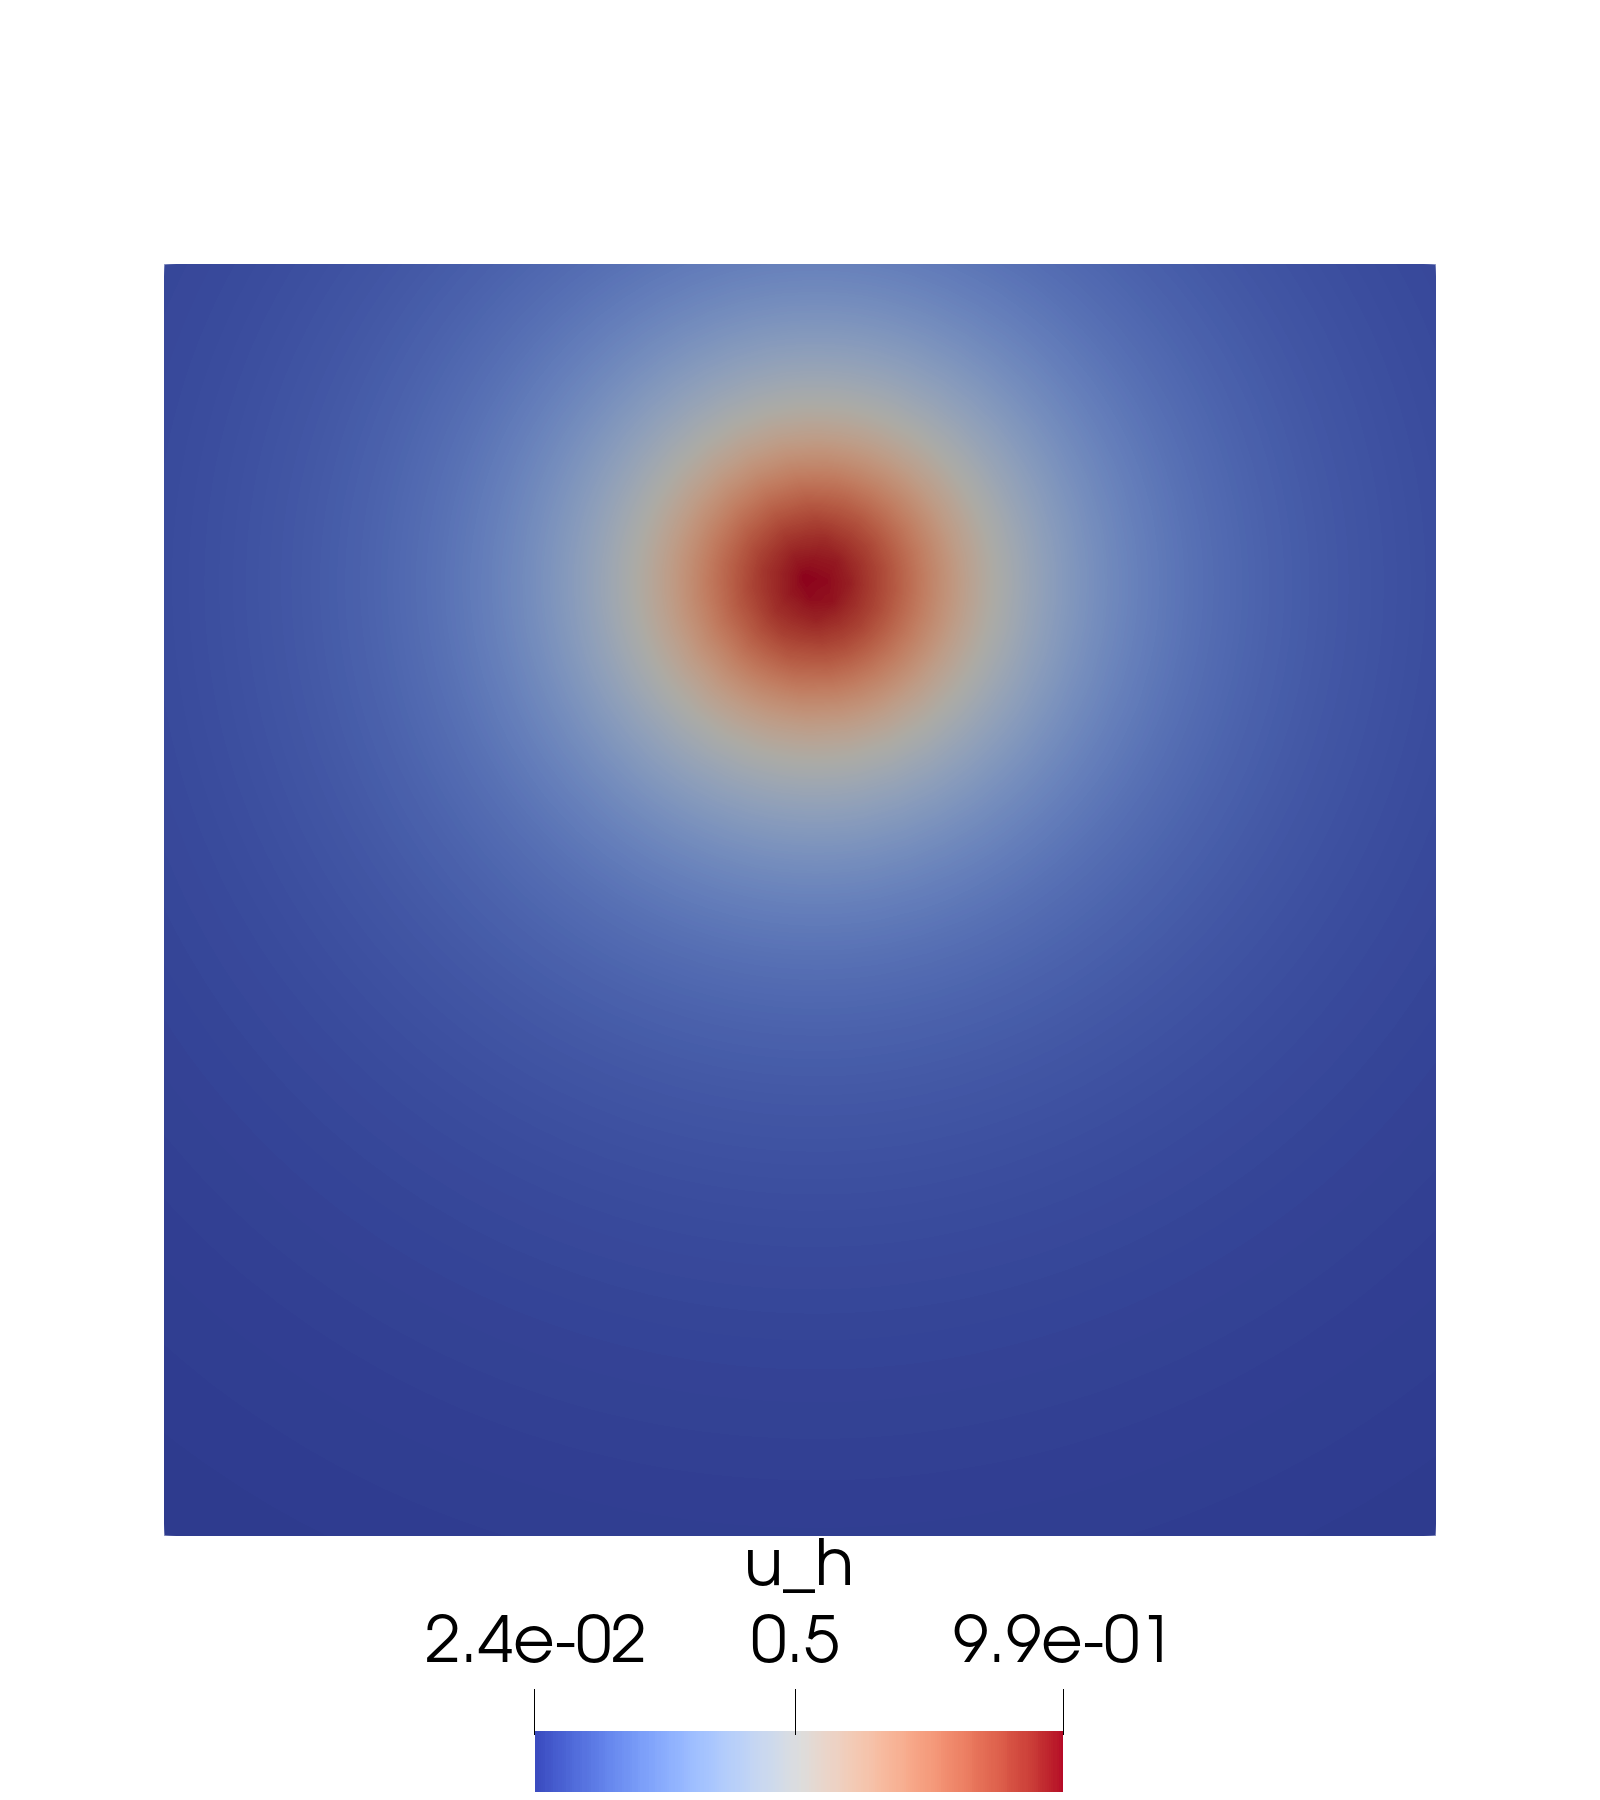
\includegraphics[width=0.24\linewidth]{figures/heat/heat_sol.0000.png} &
            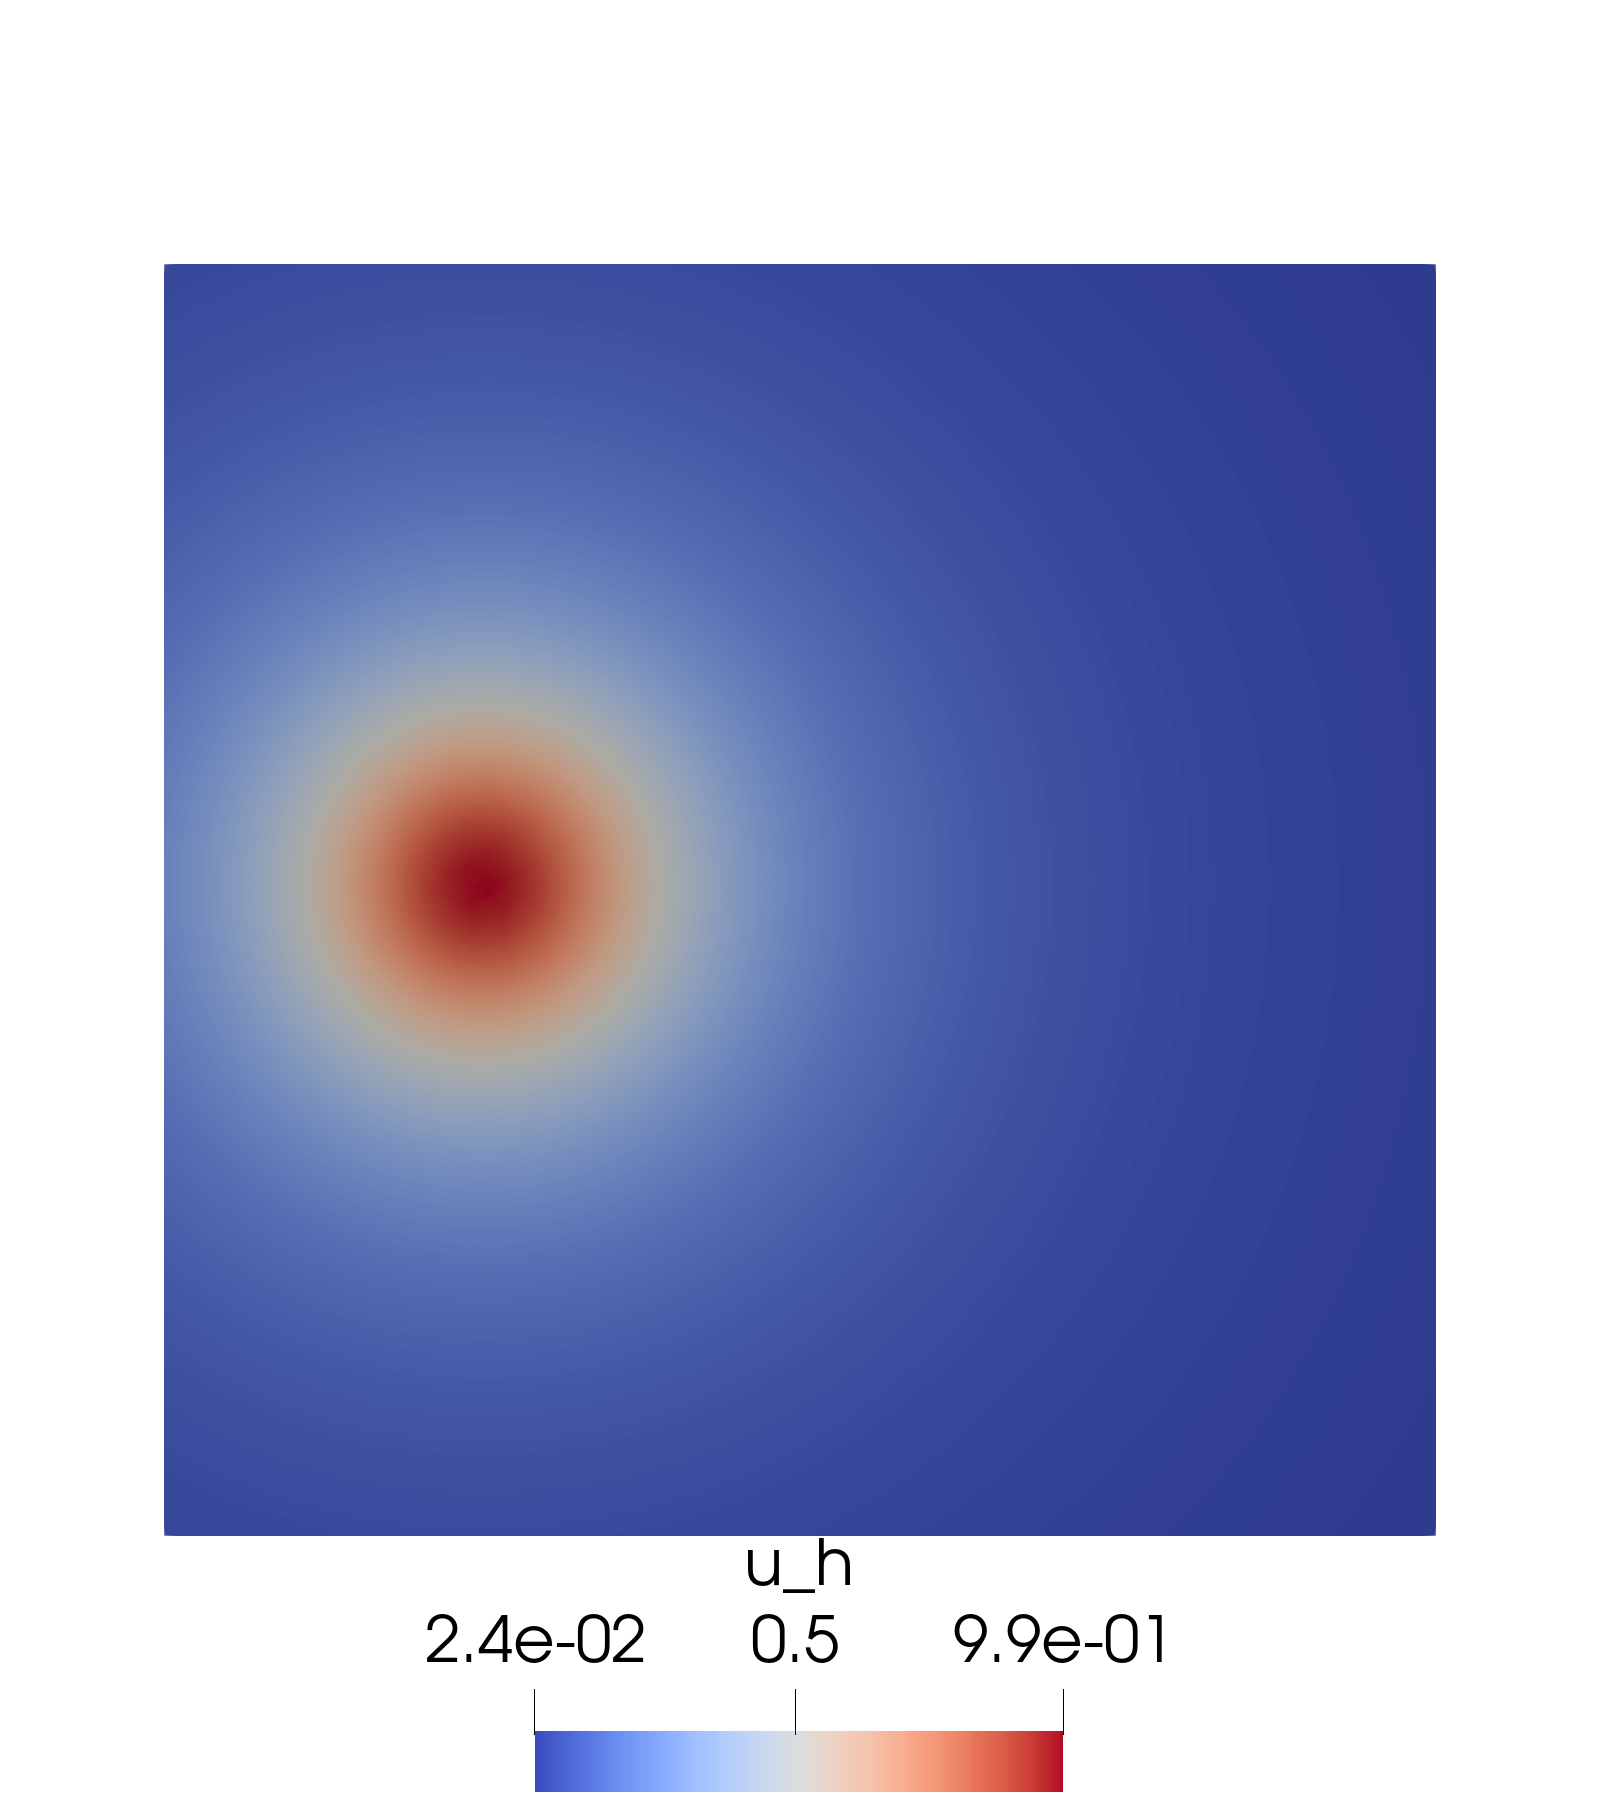
\includegraphics[width=0.24\linewidth]{figures/heat/heat_sol.0001.png} &
            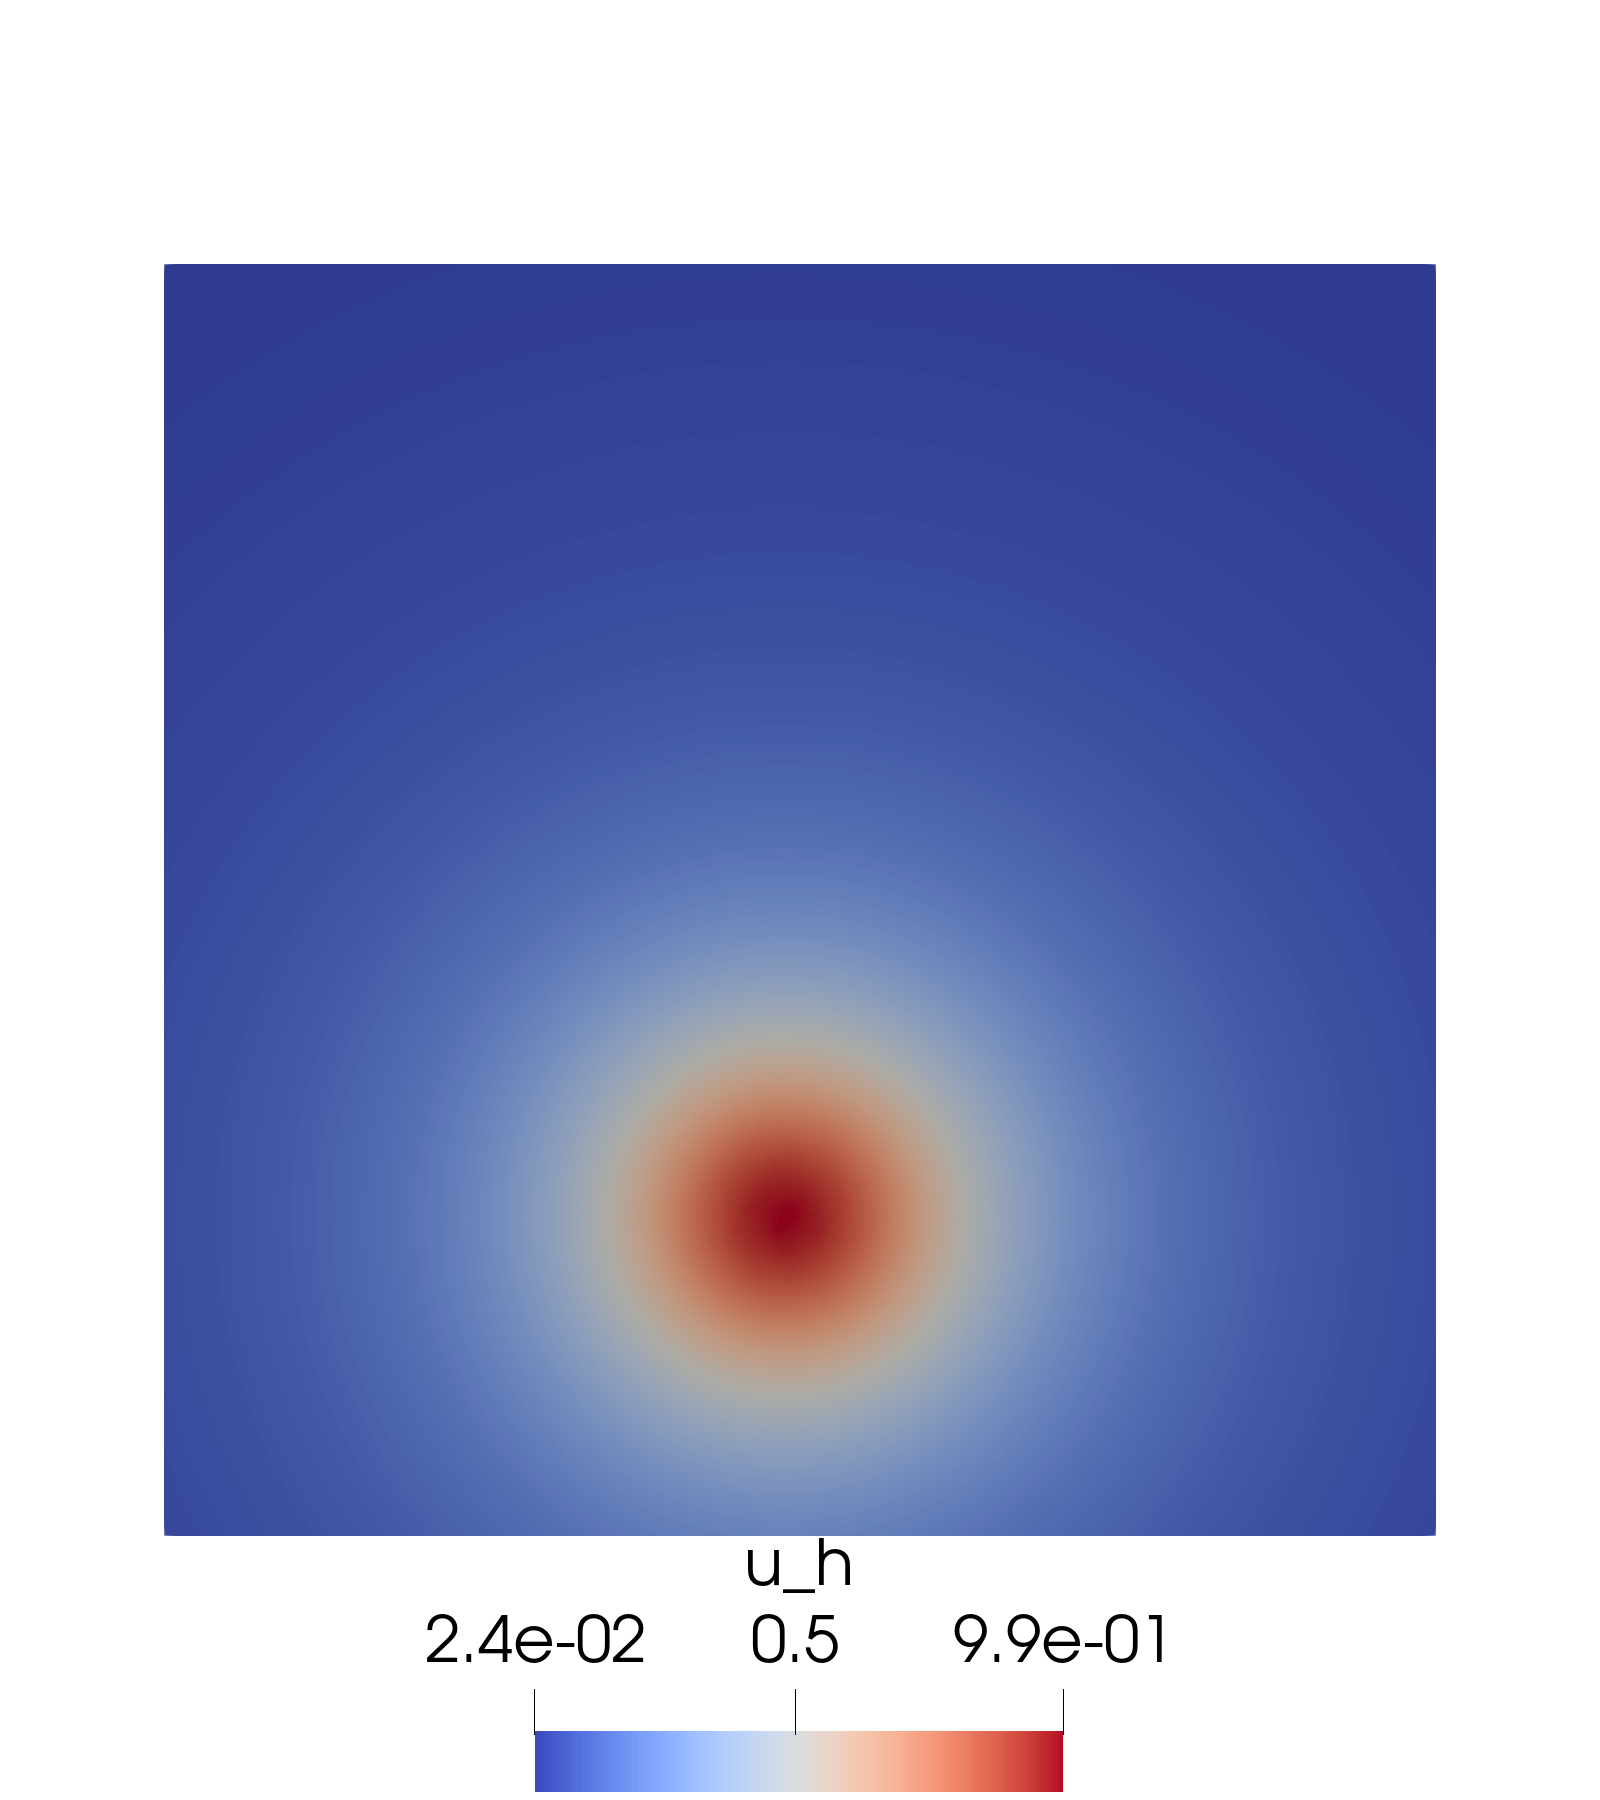
\includegraphics[width=0.24\linewidth]{figures/heat/heat_sol.0002.png} &
            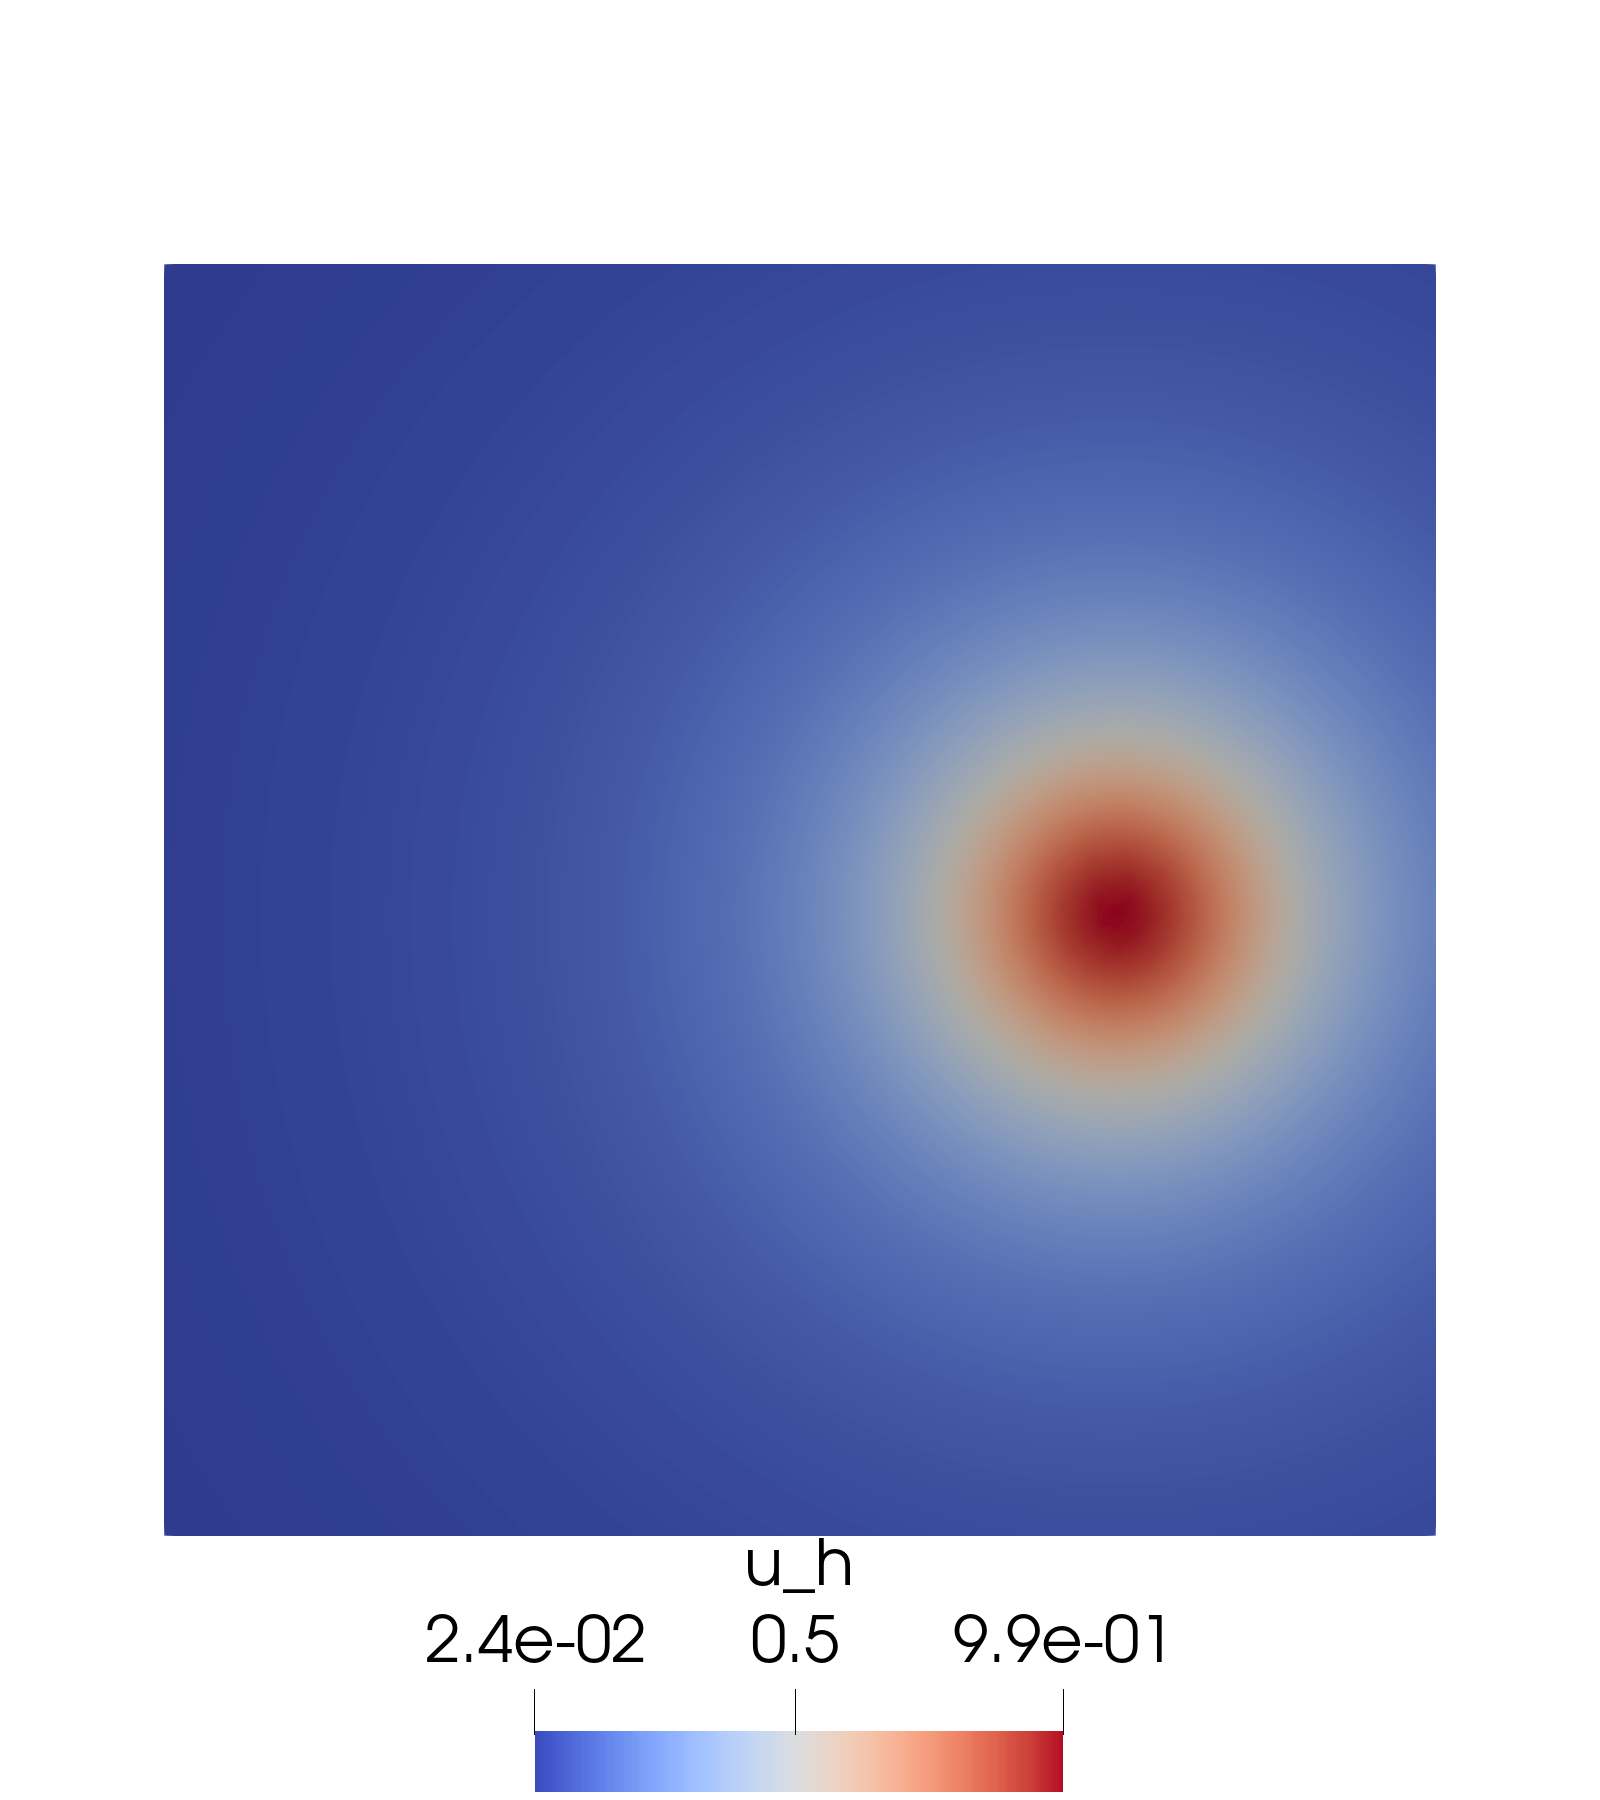
\includegraphics[width=0.24\linewidth]{figures/heat/heat_sol.0003.png}
        \end{tabular}
        \caption{Numerical rotating-hill solution.}
        \label{fig:moving-hill-solution}
    \end{subfigure}

    \vspace{6pt}

    % Row 2: strong-residual meshes
    \begin{subfigure}{\textwidth}
        \centering
        \begin{tabular}{@{}cccc@{}}
            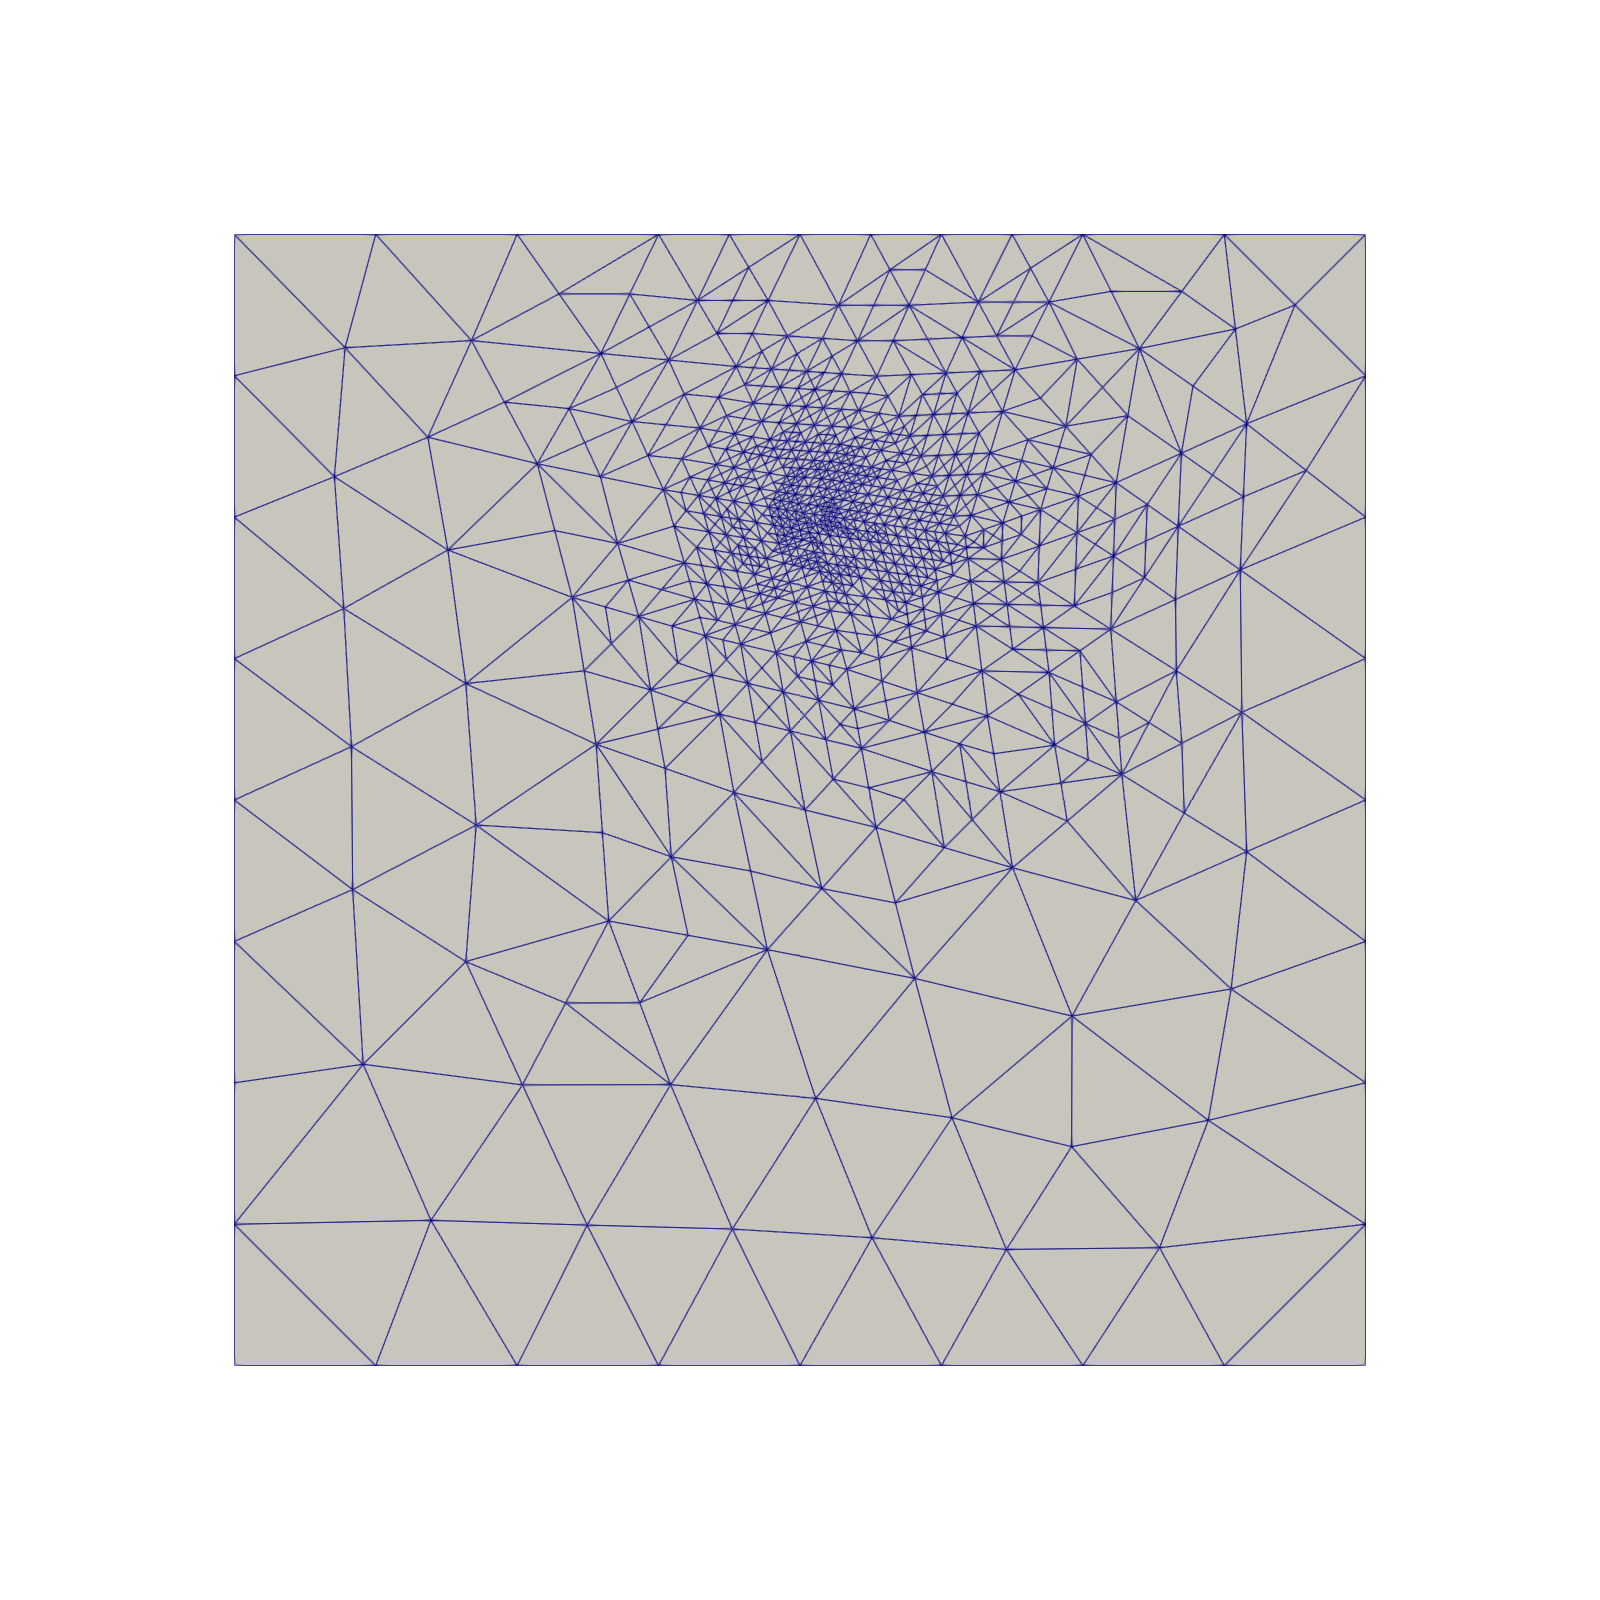
\includegraphics[width=0.24\linewidth]{figures/heat/heat_strong.0000.png} &
            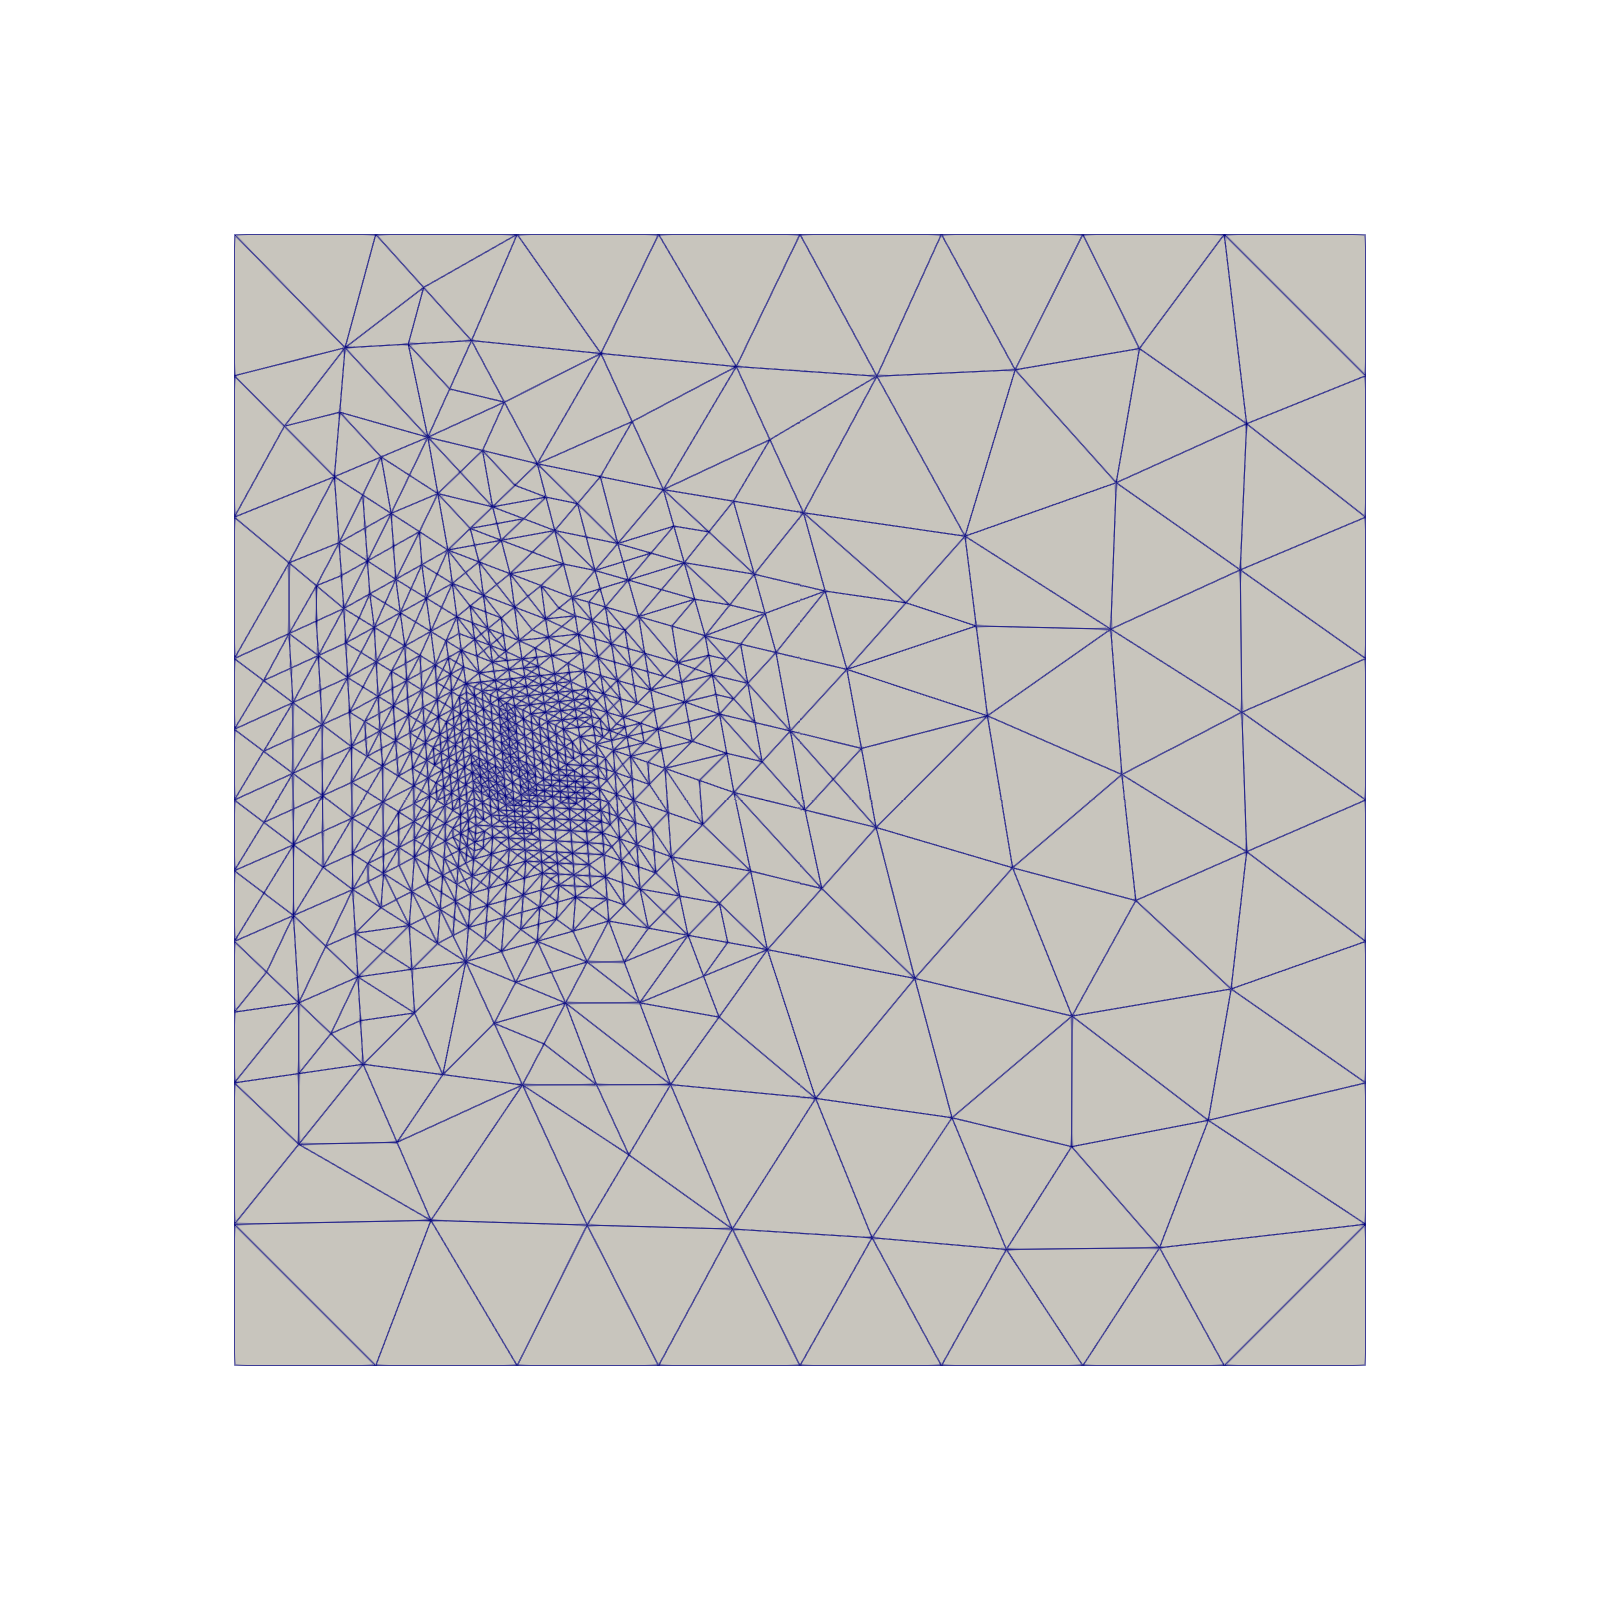
\includegraphics[width=0.24\linewidth]{figures/heat/heat_strong.0001.png} &
            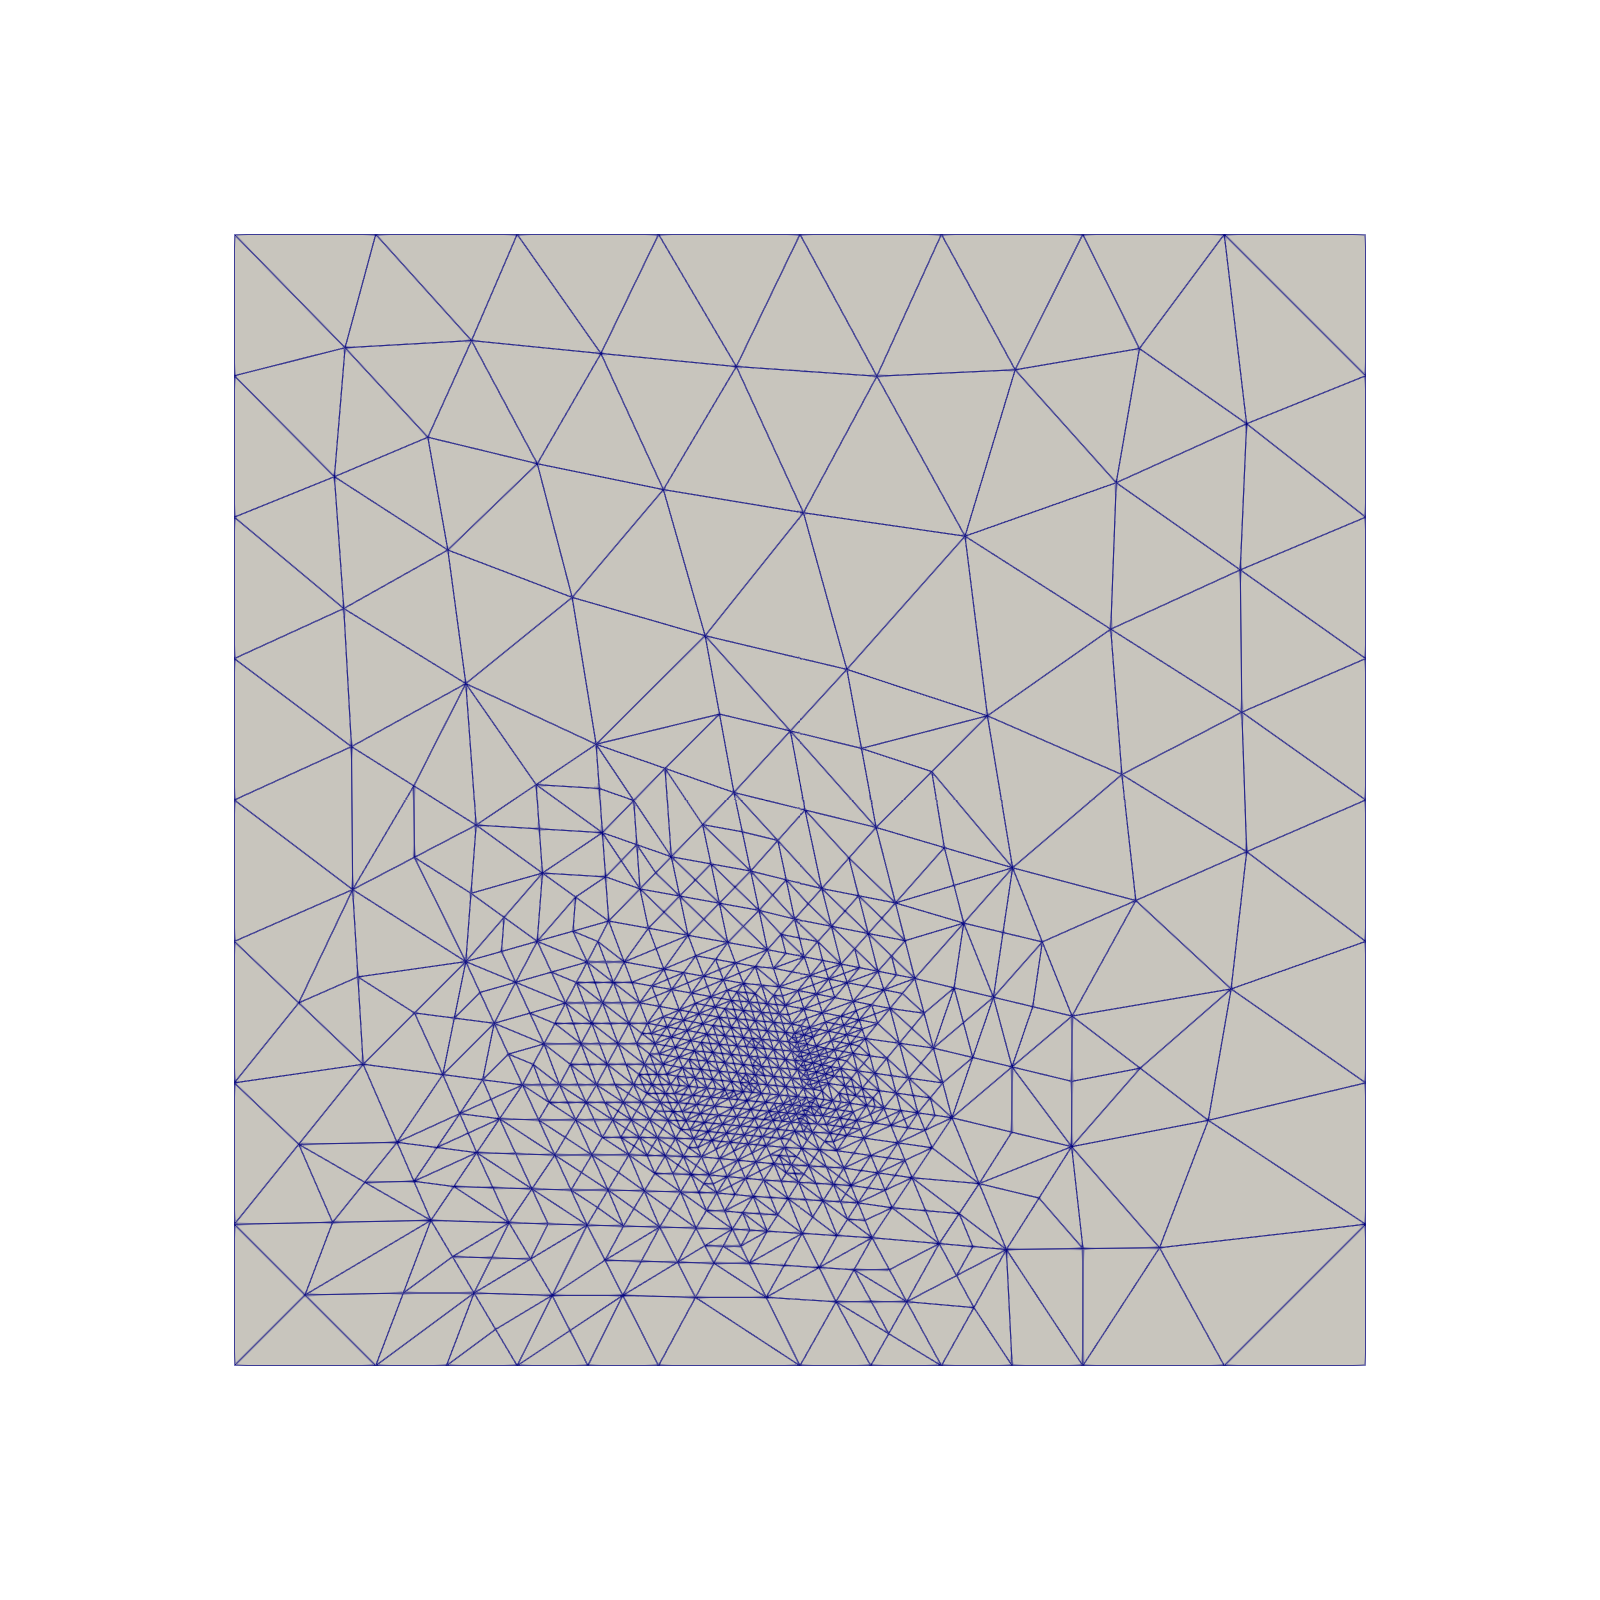
\includegraphics[width=0.24\linewidth]{figures/heat/heat_strong.0002.png} &
            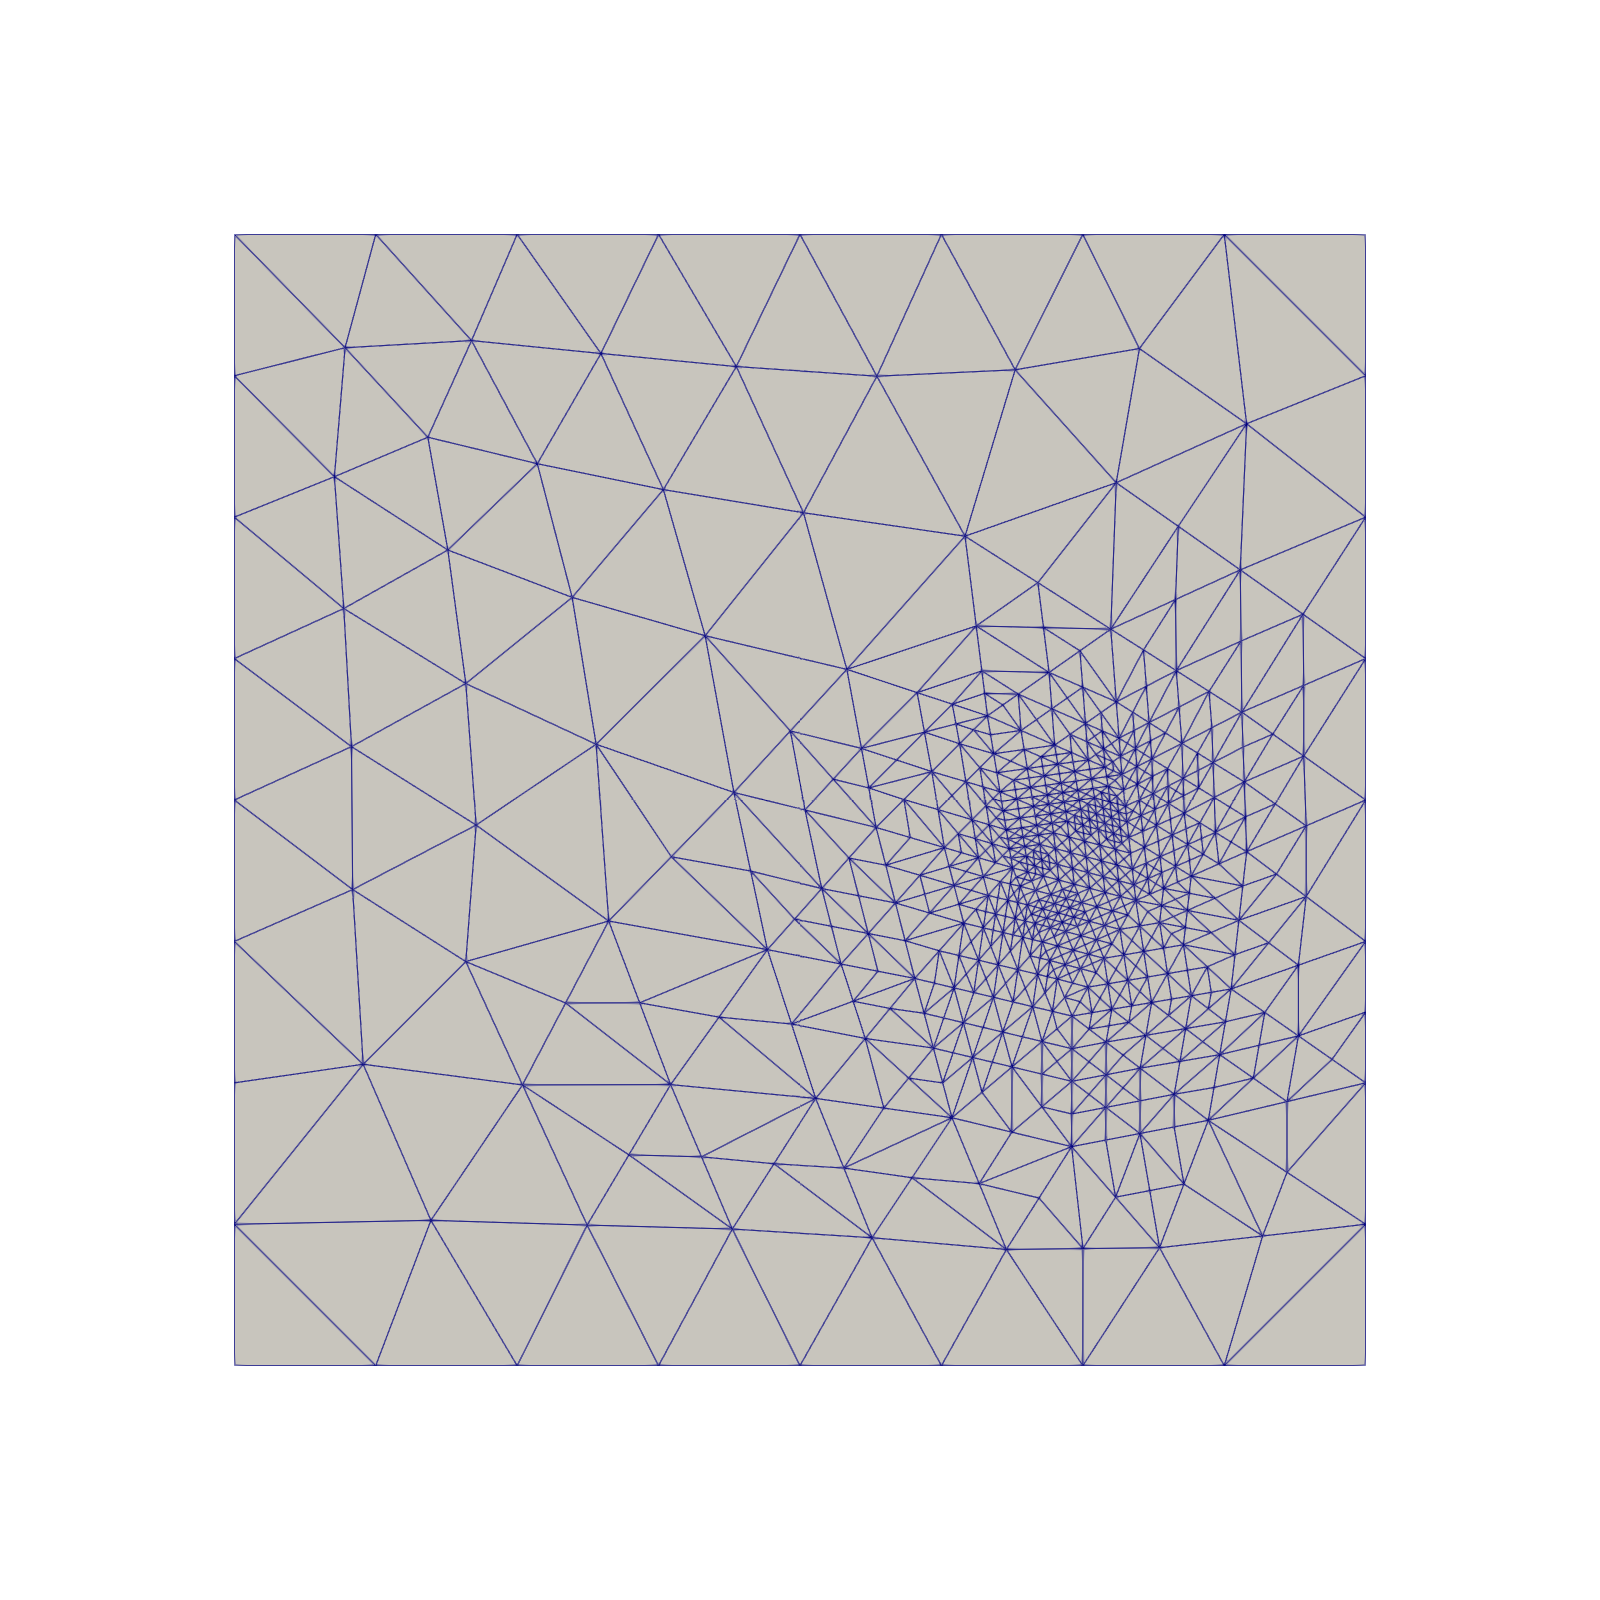
\includegraphics[width=0.24\linewidth]{figures/heat/heat_strong.0003.png}
        \end{tabular}
        \caption{Slabwise spatial meshes generated by the manual strong-residual method.}
        \label{fig:moving-hill-strong-meshes}
    \end{subfigure}

    \vspace{6pt}

    % Row 3: bubble-recovery meshes
    \begin{subfigure}{\textwidth}
        \centering
        \begin{tabular}{@{}cccc@{}}
            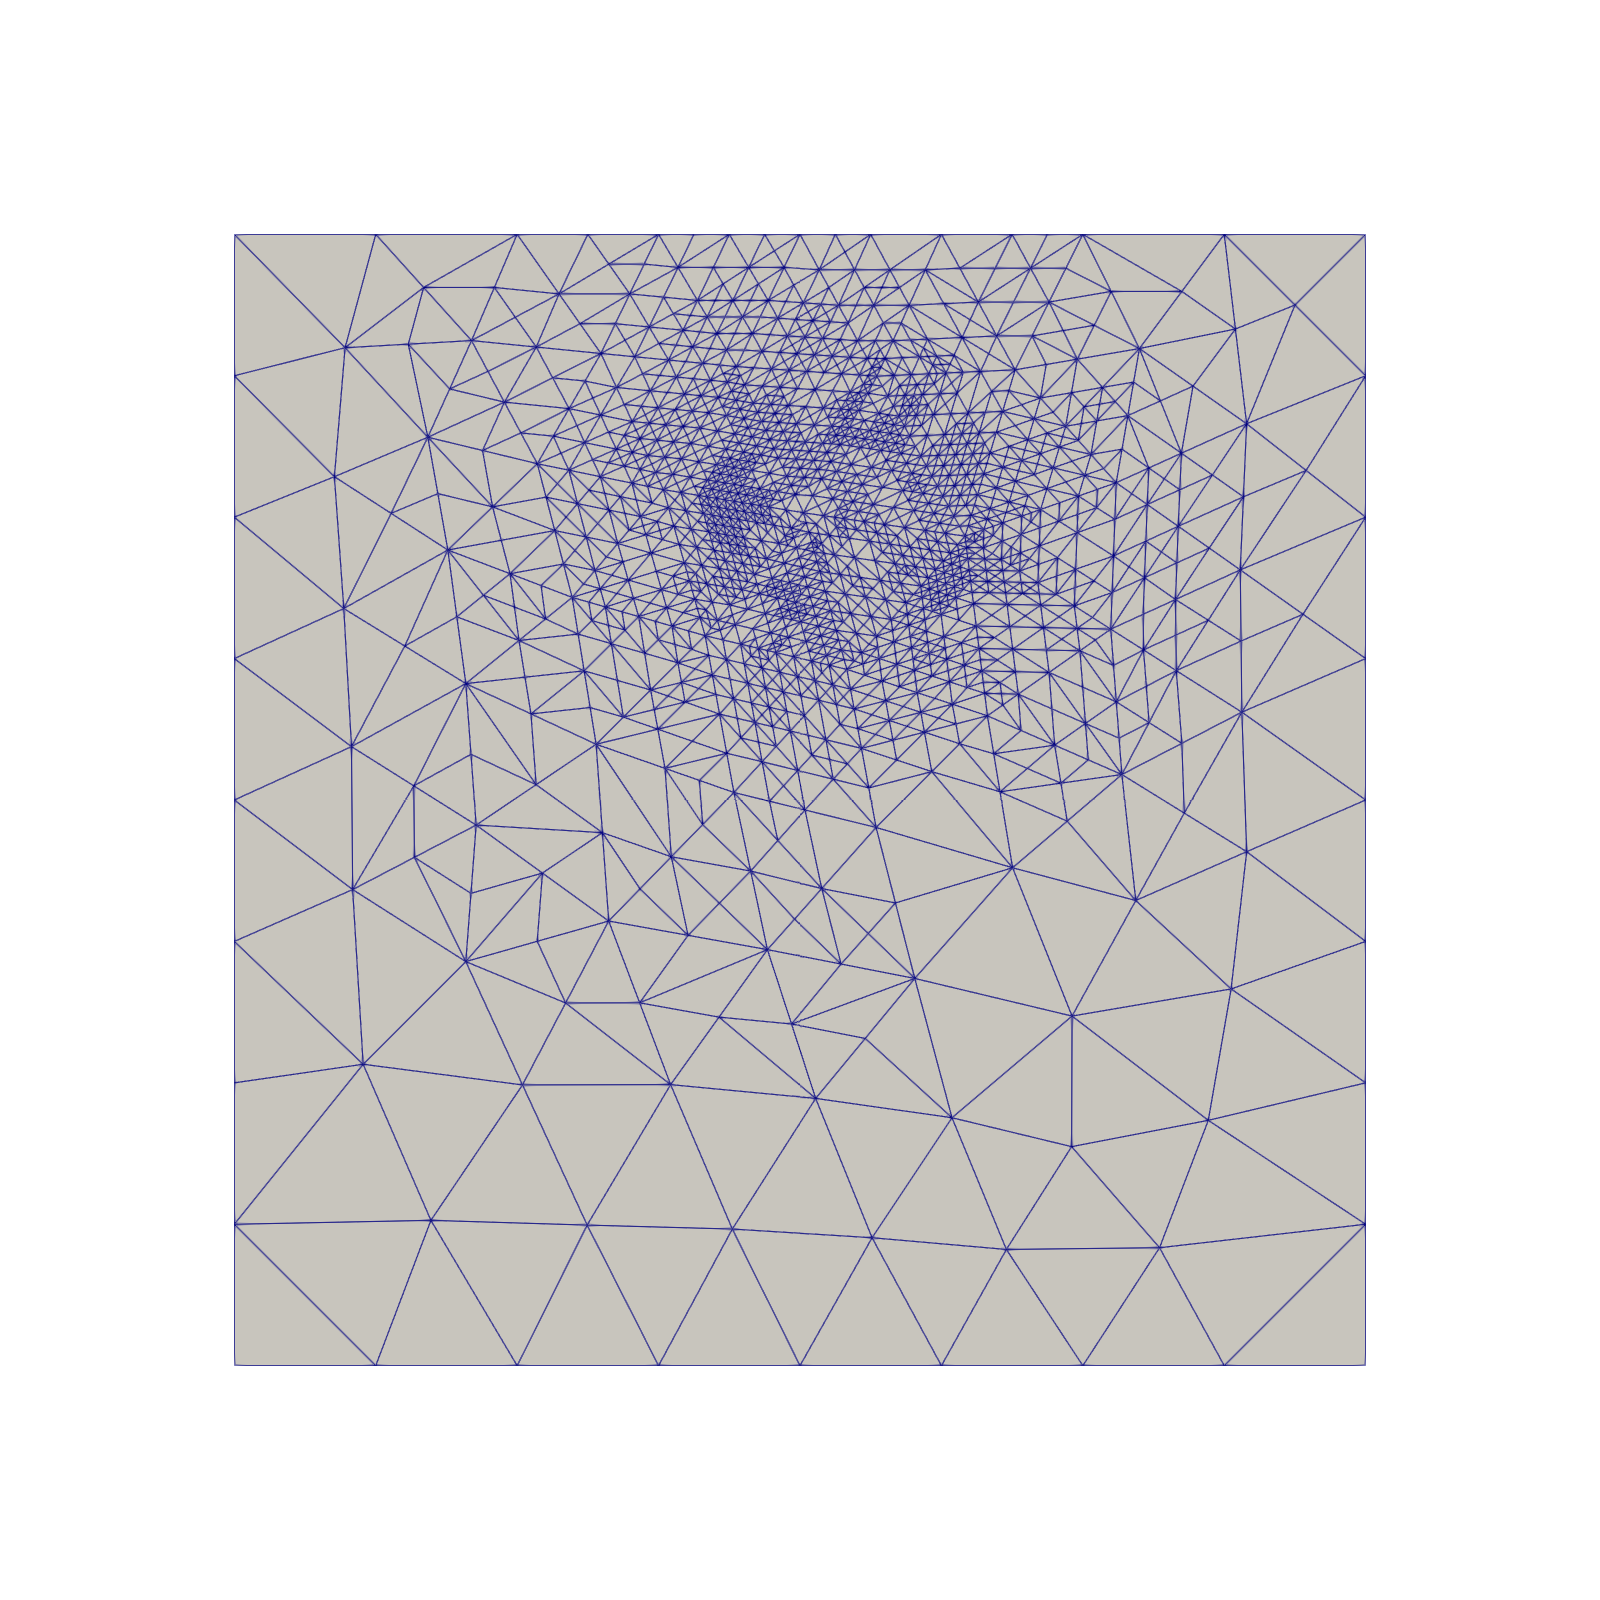
\includegraphics[width=0.24\linewidth]{figures/heat/heat_bubble.0000.png} &
            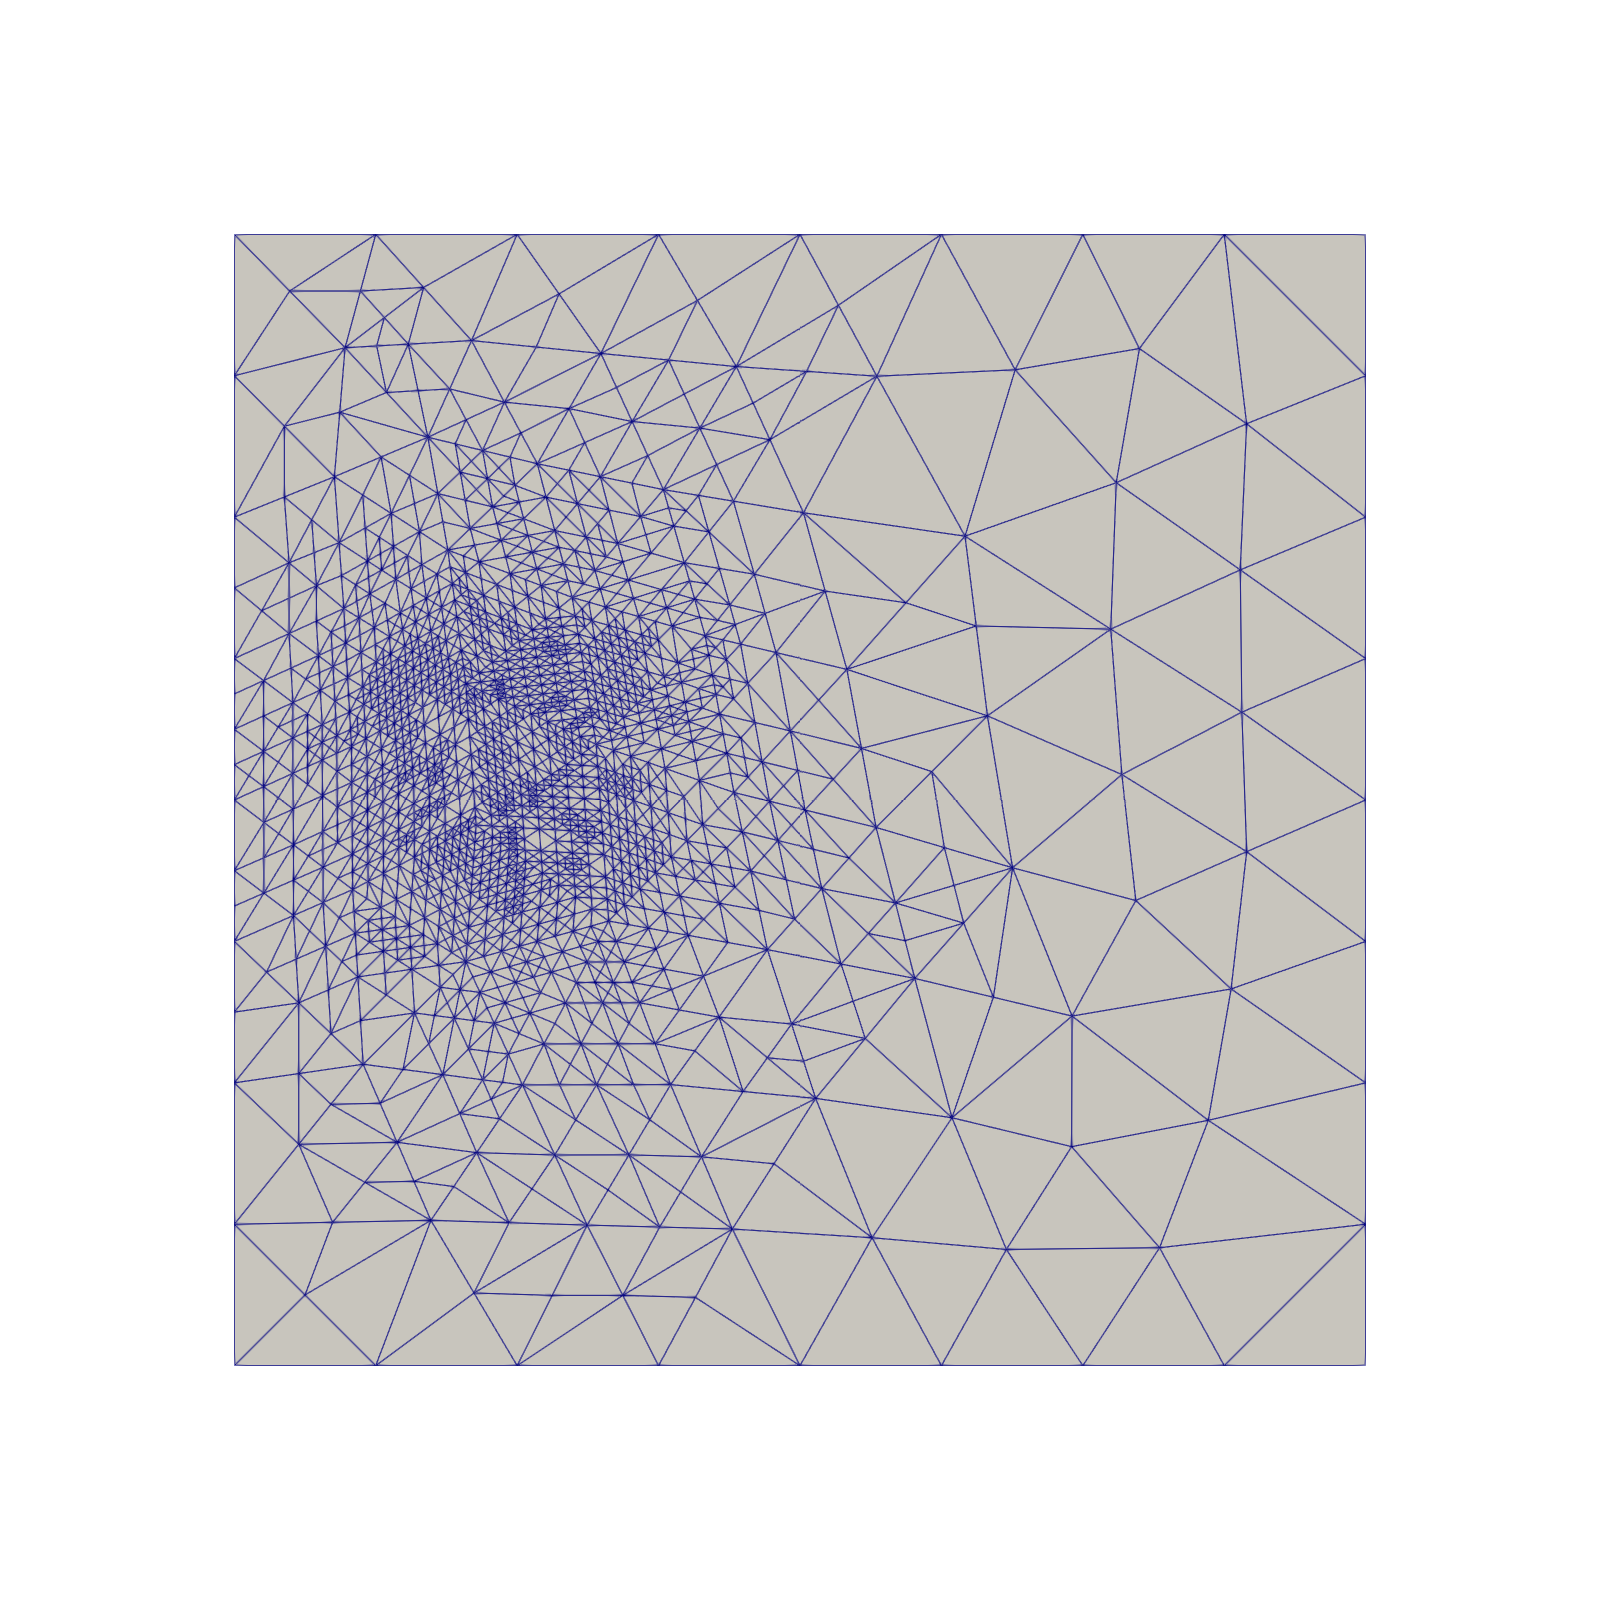
\includegraphics[width=0.24\linewidth]{figures/heat/heat_bubble.0001.png} &
            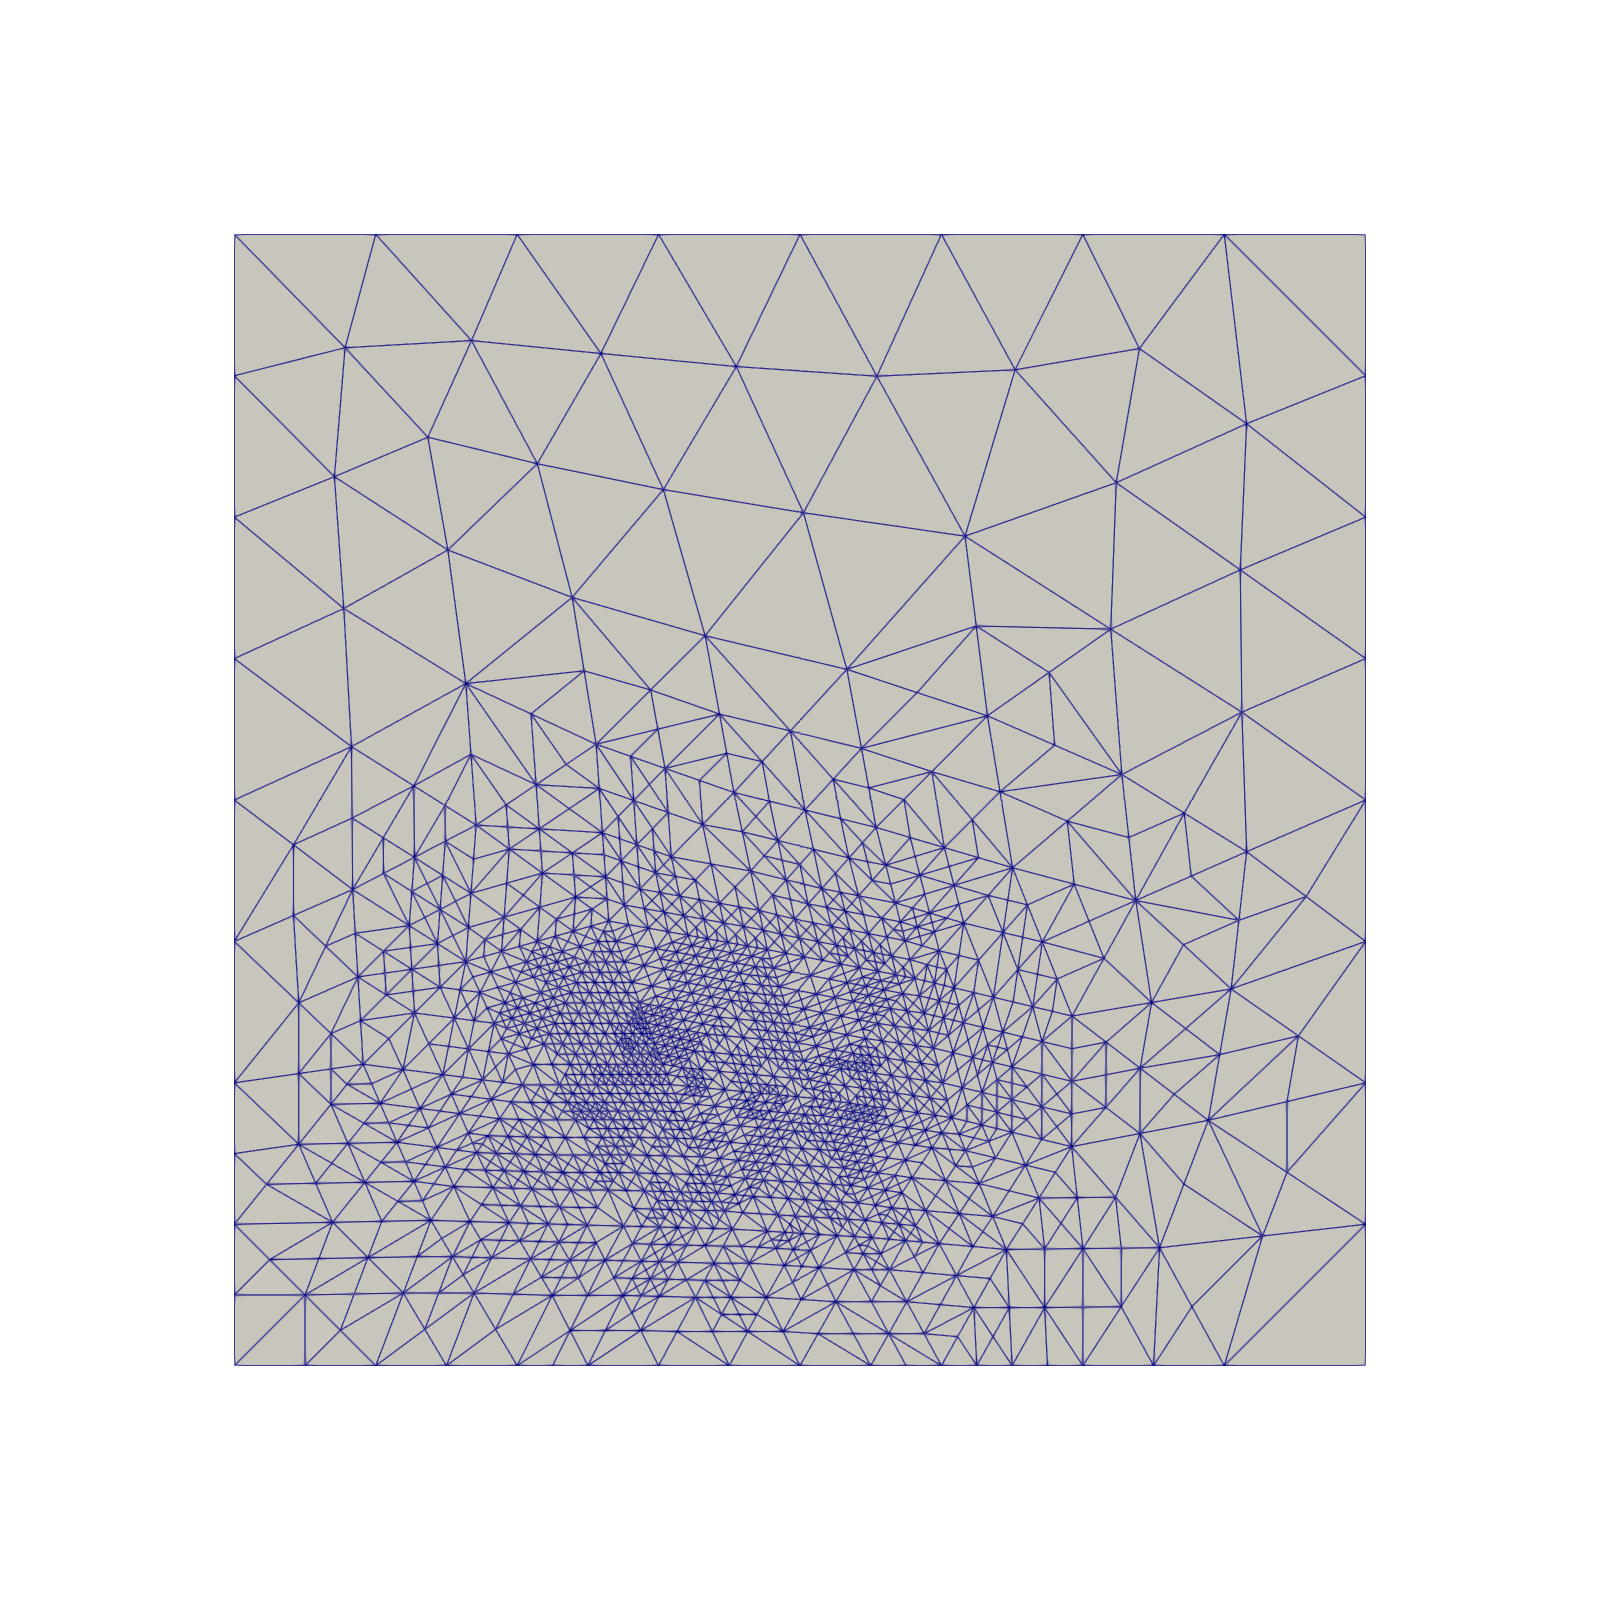
\includegraphics[width=0.24\linewidth]{figures/heat/heat_bubble.0002.png} &
            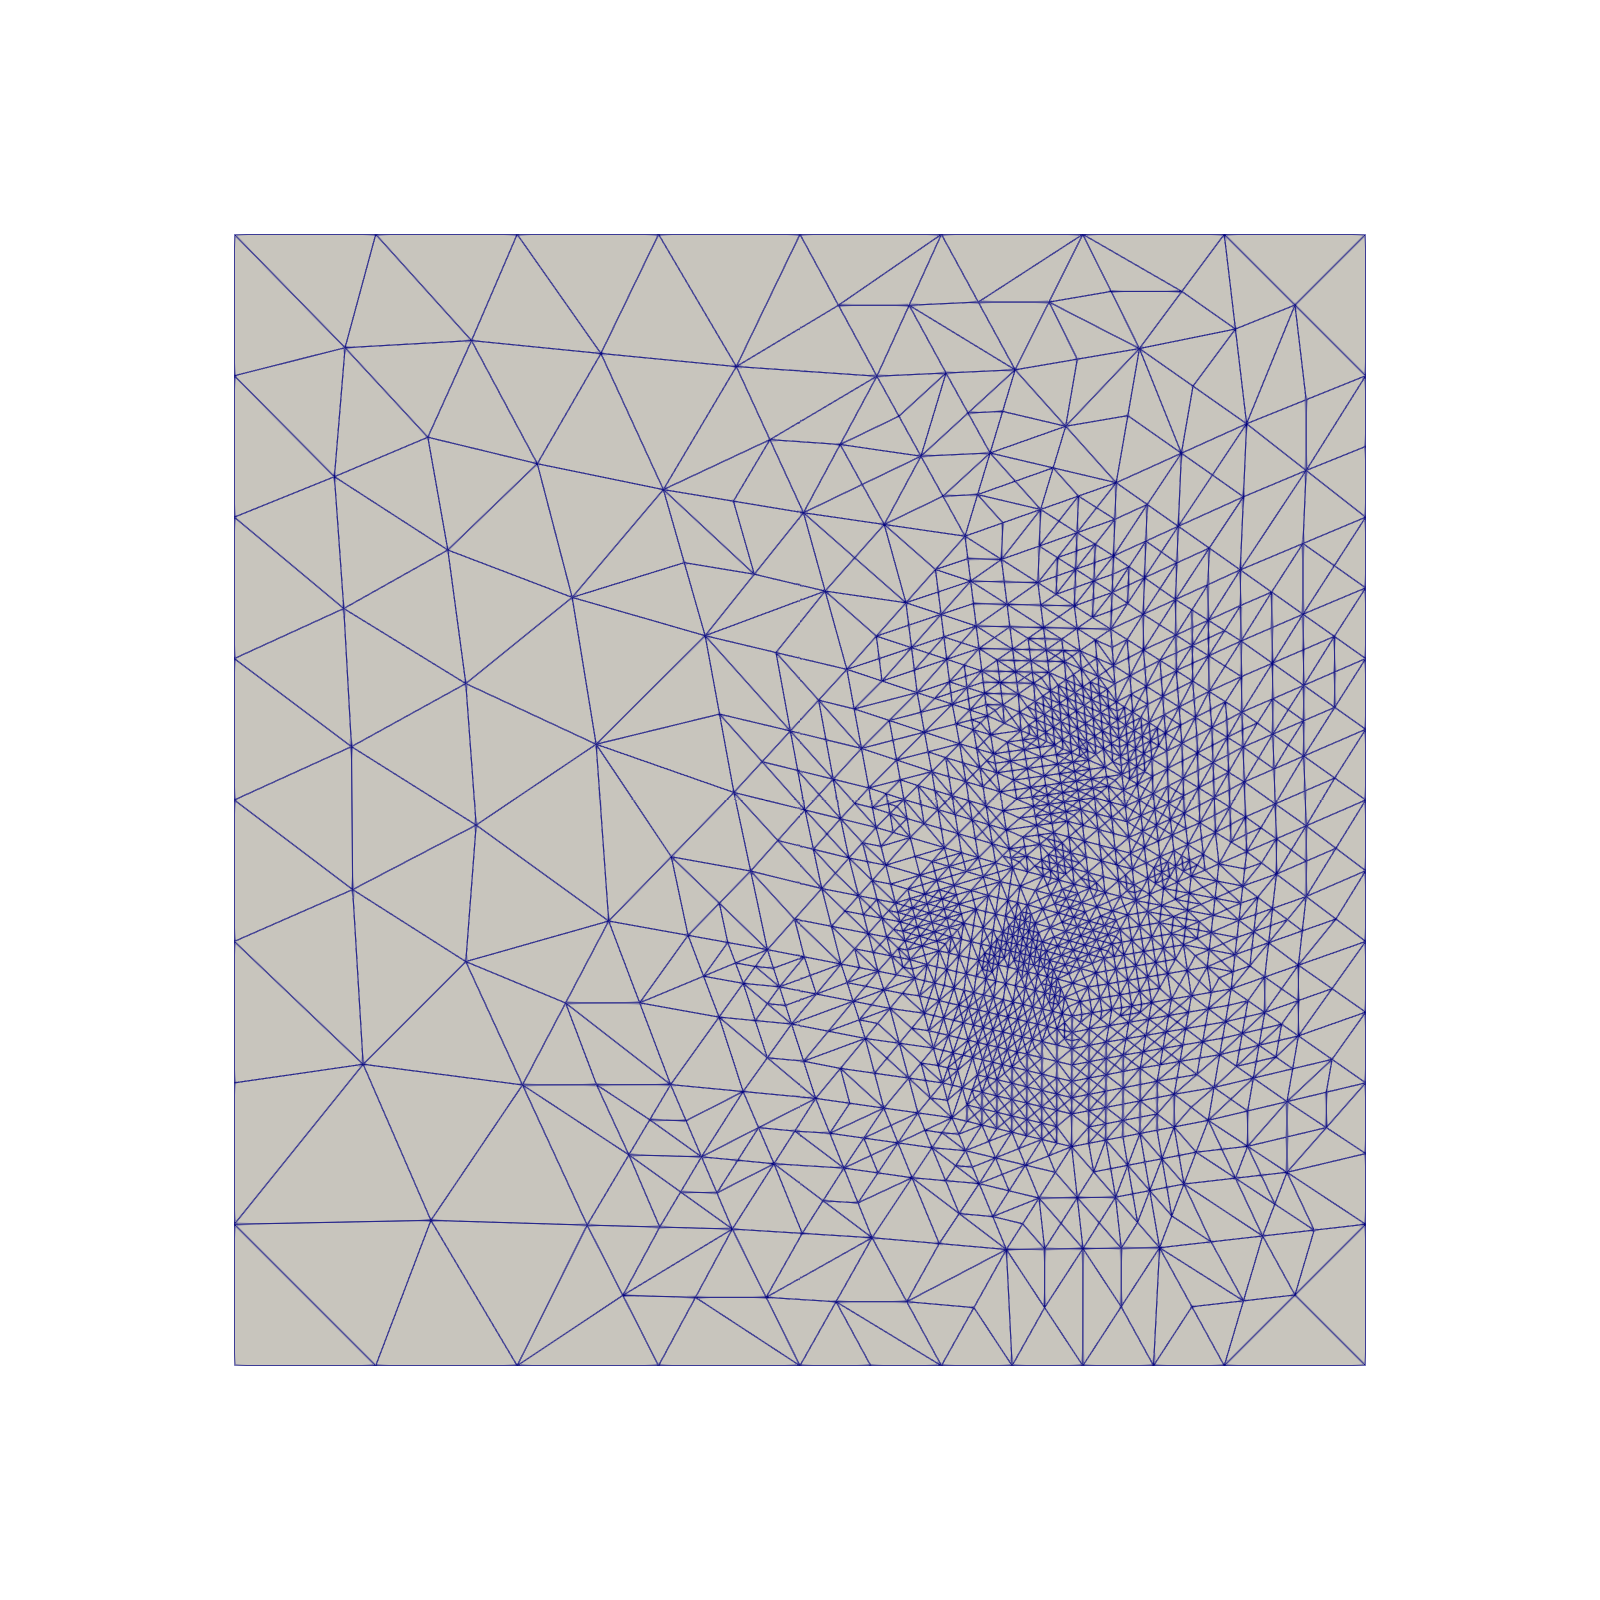
\includegraphics[width=0.24\linewidth]{figures/heat/heat_bubble.0003.png}
        \end{tabular}
        \caption{Slabwise spatial meshes generated by the automated bubble-recovery method.}
        \label{fig:moving-hill-bubble-meshes}
    \end{subfigure}

    \caption{Comparison of the numerical rotating-hill solution and the corresponding adaptive spatial meshes at iteration 6. Columns correspond to the physical snapshot times \(t=0.25\), \(0.50\), \(0.75\), and \(1.00\).}
    \label{fig:moving-hill-comparison}
\end{figure}

For both localisation methods, refinement follows the trajectory of the moving hill. The difference lies in how the activity is distributed among the space--time cells. Under the present marking rule, all space–time cell indicators are sorted in descending order and the largest entries are selected until their cumulative sum reaches \(\theta=0.40\) of the total indicator activity. The strong-residual indicator is a positive upper bound. Therefore, fewer cells are selected and the resulting refined patches remain relatively compact.

By contrast, the automated indicator is formed by summing signed recovered contributions. 
These signed contributions may partially cancel, while recovered facet terms are distributed between neighbouring cells. For the present experiment, the resulting marking activity is spread over a broader part of the mesh. As a result, more cells are marked within each slab, and more slabs satisfy the \(10\%\) temporal-refinement trigger. This accounts for both the broader spatial patches visible in the snapshots and the larger number of time slabs in the automated sequence.



% It is not surprising that the strong-residual method performs slightly better than the automated method in this example. However, the results motivate a componentwise marking alternative:
% \[
% m_{K,n}^{\mathrm{comp}}
% \coloneqq
% |\eta_{\mathrm{vol}}|
% +
% |\eta_{\mathrm{spatial}}|
% +
% |\eta_{\mathrm{temporal}}|.
% \]
% This modification prevents large entity contributions from being hidden by local sign cancellation and may therefore provide a more robust refinement indicator in cases where the recovered components have competing signs. However, it may also mark unexpected regions and increase computational cost, so its benefit must be assessed experimentally rather than assumed.
%\pef{I'd suggest cutting this last bit from `It is not surprising \dots'}
